%% This file is modified by Veli Mäkinen from HY_fysiikka_LuKtemplate.tex authored by Roope Halonen ja Tomi Vainio.
%% Some text is also inherited from engl_malli.tex by Kutvonen, Erkiö, Mäkelä, Verkamo, Kurhila, and Nykänen.


% STEP 1: Choose oneside or twoside
\documentclass[english,twoside,openright]{HYgraduMLDS}
%finnish,swedish

\usepackage{lmodern} % Font package
\usepackage{textcomp} % Package for special symbols
\usepackage[pdftex]{color, graphicx} % For pdf output and jpg/png graphics
\usepackage[pdftex, plainpages=false]{hyperref} % For hyperlinks and pdf metadata
\usepackage{fancyhdr} % For nicer page headers
\usepackage{tikz} % For making vector graphics (hard to learn but powerful)
%\usepackage{wrapfig} % For nice text-wrapping figures (use at own discretion)
\usepackage{amsmath, amssymb} % For better math
\usepackage{amsthm}
%\usepackage[square]{natbib} % For bibliography
\usepackage[footnotesize,bf]{caption} % For more control over figure captions
\usepackage{blindtext}
\usepackage{titlesec}
\usepackage{booktabs}
\usepackage[titletoc]{appendix}
\usepackage[ruled, vlined]{algorithm2e}

\onehalfspacing %line spacing
%\singlespacing
%\doublespacing

%\fussy 
\sloppy % sloppy and fussy commands can be used to avoid overlong text lines

% STEP 2:
% Set up all the information for the title page and the abstract form.
% Replace parameters with your information.
\title{Differentially Private Markov Chain Monte Carlo}
\author{Ossi Räisä}
\date{\today}
\prof{Associate Professor Antti Honkela}
\censors{Associate Professor Antti Honkela}{Doctor Antti Koskela}{}
\keywords{Differential Privacy, Markov Chain Monte Carlo}
\depositeplace{}
\additionalinformation{}


\classification{\protect{\ \\
% \  General and reference $\rightarrow$ Document types  $\rightarrow$ Surveys and overviews\  \\
% \  Applied computing  $\rightarrow$ Document management and text processing  $\rightarrow$ Document management $\rightarrow$ Text editing\\
}}

% if you want to quote someone special. You can comment this line and there will be nothing on the document.
%\quoting{Bachelor's degrees make pretty good placemats if you get them laminated.}{Jeph Jacques} 


% OPTIONAL STEP: Set up properties and metadata for the pdf file that pdfLaTeX makes.
% But you don't really need to do this unless you want to.
\hypersetup{
    % bookmarks=true,         % show bookmarks bar first?
    unicode=true,           % to show non-Latin characters in Acrobat’s bookmarks
    pdftoolbar=true,        % show Acrobat’s toolbar?
    pdfmenubar=true,        % show Acrobat’s menu?
    pdffitwindow=false,     % window fit to page when opened
    pdfstartview={FitH},    % fits the width of the page to the window
    pdftitle={},            % title
    pdfauthor={},           % author
    pdfsubject={},          % subject of the document
    pdfcreator={},          % creator of the document
    pdfproducer={pdfLaTeX}, % producer of the document
    pdfkeywords={something} {something else}, % list of keywords for
    pdfnewwindow=true,      % links in new window
    colorlinks=true,        % false: boxed links; true: colored links
    linkcolor=blue,        % color of internal links
    citecolor=blue,        % color of links to bibliography
    filecolor=magenta,      % color of file links
    urlcolor=cyan           % color of external links
}

\newtheorem{lemma}{Lemma}
\newtheorem{theorem}{Theorem}
\newtheorem{definition}{Definition}

\newcommand{\R}{\mathbb{R}}
\newcommand{\Z}{\mathbb{Z}}
\newcommand{\Q}{\mathbb{Q}}
\newcommand{\N}{\mathbb{N}}
\newcommand{\cl}[1]{\overline{#1}}
\newcommand{\kl}{D_{\mathrm{KL}}}
\newcommand{\dmid}{\mid\mid}
\newcommand{\var}{\mathrm{Var}}
\newcommand{\dx}{\mathrm{d}}
\newcommand{\calm}{{\mathcal{M}}}
\newcommand{\calx}{{\mathcal{X}}}
\newcommand{\calu}{{\mathcal{U}}}
\newcommand{\caln}{{\mathcal{N}}}
\newcommand{\call}{{\mathcal{L}}}
\newcommand{\caly}{{\mathcal{Y}}}
\DeclareMathOperator{\erfc}{erfc}
\DeclareMathOperator{\ban}{Ban}
\DeclareMathOperator{\diag}{diag}
\DeclareMathOperator{\clip}{clip}

\begin{document}

% Generate title page.
\maketitle

% STEP 3:
% Write your abstract (of course you really do this last).
% You can make several abstract pages (if you want it in different languages),
% but you should also then redefine some of the above parameters in the proper
% language as well, in between the abstract definitions.

\begin{abstract}
 
\end{abstract}

% Place ToC
\mytableofcontents

\mynomenclature

% -----------------------------------------------------------------------------------
% STEP 4: Write the thesis.
% Your actual text starts here. You shouldn't mess with the code above the line except
% to change the parameters. Removing the abstract and ToC commands will mess up stuff.
\chapter{Introduction}

\chapter{Background}

This chapter covers the basics of differential privacy, Bayesian inference
and Markov chain Monte Carlo algorithms needed in the later chapters. To keep
the introduction brief, only directly needed concepts are covered, and much
of the motivation behind the subjects is left out.

\section{Differential Privacy}\label{DP_background}
\emph{Differential privacy} (DP)~\cite{DMN06, DwR14} is a property of
an algorithm that quantifies the
amount of information about private data an adversary can gain from the 
publication of the algorithm's output.
The most commonly used definition uses two real numbers, 
\(\epsilon\) and \(\delta\), to quantify the information gain, or, from the 
perspective of a data subject, the privacy loss of the algorithm.
DP algorithms must necessarily\footnote{Unless the algorithm does not
actually use the private data.} include randomness to mask influence of the
private data, so all of the considered algorithms in this thesis are randomised.
DP randomised algorithms are also called \emph{mechanisms} in this thesis, and in the
DP literature.

The most common definition is called \((\epsilon, \delta)\)-approximate
differential privacy (ADP)~\cite{DKM06, DwR14}.
The case where \(\delta = 0\) is called \(\epsilon\)-DP or 
pure DP.

\begin{definition}\label{ADP-definition}
    A mechanism \(\calm\colon \calx \to \calu\) is \((\epsilon, \delta)\)-ADP if
    for all neighbouring inputs \(x\in \calx\) and \(x'\in \calx\) and 
    all measurable sets \(S \subset \calu\)
    \[
        P(\calm(x)\in S) \leq e^\epsilon P(\calm(x')\in S) + \delta.
    \]
\end{definition}

The neighbourhood relation in the definition is domain specific. With tabular 
data the most common definitions are the add/remove neighbourhood and 
substitute neighbourhood.
\begin{definition}
    Two tabular datasets are said to be add/remove neighbours if they are equal 
    after adding or removing at most one row to or from one of them. The datasets 
    are said to be in substitute neighbours if they are equal after 
    changing at most one row in one of them.
\end{definition}
The neighbourhood relation is denoted by \(\sim\). The definitions and 
theorems of this section are valid for all neighbourhood relations.

There many other definitions of differential privacy that are mostly used
to compute \((\epsilon, \delta)\)-bounds for ADP. This thesis uses two of them: 
Rényi-DP (RDP)~\cite{Mironov17} and 
zero-concentrated differential privacy (zCDP)~\cite{BuS16}. Both are based 
on Rényi divergence~\cite{Mironov17}, which is a particular way of 
measuring the distance\footnote{
  Statistical divergences are commonly called distances, even though they
  typically are not metrics.
} between random variables.

\begin{definition}
    For random variables with density or probability mass functions 
    \(P\) and \(Q\) the Rényi divergence of order 
    \(1 < \alpha < \infty\) is
    \[
        D_\alpha(P\dmid Q) = \frac{1}{\alpha - 1}\ln E_{x\sim Q}
        \left(\frac{P(x)^\alpha}{Q(x)^\alpha}\right).
    \]
    Orders \(\alpha = 1\) and \(\alpha = \infty\) are defined 
    by continuity:
    \[
        D_1(P\dmid Q) = \lim_{\alpha \to 1-} D_\alpha(P\dmid Q),
    \]
    \[
        D_\infty(P \dmid Q) = \lim_{\alpha\to \infty}D_\alpha(P\dmid Q).
    \]
\end{definition}

Both Rényi-DP and zCDP can be expressed as bounds on the 
Rényi divergence between the outputs of a randomised algorithm with
neighbouring inputs:

\begin{definition}
    A mechanism \(\calm\) is \((\alpha, \epsilon)\)-Rényi DP
    if for all \(x \sim x'\)
    \[
        D_\alpha(\calm(x)\dmid \calm(x')) \leq \epsilon.
    \]
    \(\calm\) is \(\rho\)-zCDP if for all \(\alpha > 1\)
    and all \(x \sim x'\)
    \[
        D_\alpha(\calm(x)\dmid \calm(x')) \leq \rho \alpha.
    \]

\end{definition}

Rényi-DP and zCDP bounds can be converted to ADP bounds~\cite{Mironov17, BuS16}:
\begin{theorem}\label{other_dp_to_adp}
    If \(\calm\) is \((\alpha, \epsilon)\)-RDP, \(\calm\) is also 
    \((\epsilon - \frac{\ln \delta}{\alpha - 1}, \delta)\)-ADP for any 
    \(0 < \delta < 1\). If \(\calm\) is \(\rho\)-zCDP, \(\calm\) is also 
    \((\rho + \sqrt{-4\rho\ln \delta}, \delta)\)-ADP for any \(0 < \delta < 1\).
\end{theorem}

A very useful property of all of these definitions is composition~\cite{DwR14}: 
if mechanisms \(\calm\) and \(\calm'\) are DP, the mechanism first computing
\(\calm\) and then \(\calm'\), outputting both results, 
is also DP, although with worse bounds.
More precisely:

\begin{definition}\label{composition_definition}
    Let \(\calm\colon \calx \to \calu\) and 
    \(\calm'\colon \calx\times \calu \to \calu'\) be mechanisms.
    Their composition is the mechanism outputting
    \((\calm(x), \calm'(x, \calm(x)))\) for input \(x\).
\end{definition}

\begin{theorem}\label{composition-theorem}
    Let \(\calm\colon \calx \to \calu\) and 
    \(\calm\colon \calx\times \calu \to \calu'\) be mechanisms. Then
    \begin{enumerate}
        \item 
            If \(\calm\) is \((\epsilon, \delta)\)-ADP and 
            \(\calm'\) is \((\epsilon', \delta')\)-ADP, then 
            their composition is 
            \((\epsilon + \epsilon', \delta + \delta')\)-ADP~\cite{DKM06}
        \item 
            If \(\calm\) is \((\alpha, \epsilon)\)-RDP and 
            \(\calm'\) is \((\alpha, \epsilon')\)-RDP, then 
            their composition is \((\alpha, \epsilon + \epsilon')\)-RDP~\cite{Mironov17}
        \item 
            If \(\calm\) is \(\rho\)-zCDP and 
            \(\calm'\) is \(\rho'\)-zCDP, then 
            their composition is \((\rho + \rho')\)-zCDP~\cite{BuS16}
    \end{enumerate}
\end{theorem}

All of the composition results can be extended to any number of compositions 
by induction. Note that any step of the composition can depend on the results 
of the previous steps, not only on the private data. There are also other composition
theorems for ADP that trade increased \(\delta\) for decreased \(\epsilon\)
or vice-versa, but this thesis does not apply them directly.

As any randomised algorithm that does not use private data in any way is
\((0, 0)\)-ADP, 0-zCDP and \((\alpha, 0)\)-RDP with all \(\alpha\), 
Theorem~\ref{composition-theorem} has the following corollary, called 
post-processing immunity:

\begin{theorem}
  Let \(\calm\colon \calx\to \calu\) be an \((\epsilon, \delta)\)-ADP,
  \((\alpha, \epsilon)\)-RDP or \(\rho\)-zCDP mechanism.
  Let \(f\colon \calu\to \calu'\) be any randomised algorithm
  not using the private data. Then the composition of \(\calm\) and \(f\)
  is \((\epsilon, \delta)\)-ADP, \((\alpha, \epsilon)\)-RDP or \(\rho\)-zCDP.
\end{theorem}

There are many different DP mechanisms that are commonly used~\cite{DwR14}.
This thesis only requires one of the most commonly 
used ones: the Gaussian mechanism~\cite{DKM06}.
\begin{definition}
  The Gaussian mechanism with parameter \(\sigma^2\) is a randomised algorithm that,
  with input data \(x\) and query \(f\colon \calx\to \R^{d}\), outputs a sample from
  \(\caln(f(x), \sigma^2)\), where \(\caln\) denotes the normal distribution.
\end{definition}

The privacy bounds of the Gaussian mechanism require that the values of the
query \(f\) do not vary too much for neighbouring inputs. This requirement
is formalised as a bound on the \emph{sensitivity} of \(f\).
\begin{definition}
    The \(l_p\)-sensitivity \(\Delta_p\), with neighbourhood relation \(\sim\),
    of a function \(f\colon \calx \to \R^d\)
    is
    \[
        \Delta_p f = \sup_{x\sim x'}||f(x) - f(x')||_p.
    \]
\end{definition}

The RDP and zCDP bounds for the Gaussian 
mechanism are quite simple. The ADP bound is more complicated:

\begin{theorem}\label{gauss-DP-bounds}
    If \(\Delta_{2}f \leq \Delta\), the Gaussian mechanism is
    \begin{enumerate}
        \item 
            \((\alpha, \frac{\alpha \Delta^2}{2\sigma^2})\)-RDP~\cite{Mironov17}
        \item 
            \(\frac{\Delta^2}{2\sigma^2}\)-zCDP~\cite{BuS16}
        \item 
            \(k\) compositions of the Gaussian mechanism, with
            queries \(f_{i}\), where \(\Delta_{2}f_{i}\leq \Delta\) for
            \(1\leq i \leq k\), are
            \((\epsilon, \delta(\epsilon))\)-ADP~\cite{Sommer2019} with 
            \[
                \delta(\epsilon) 
                = \frac{1}{2}\left(
                    \erfc\left(\frac{\sigma(\epsilon - k\mu)}{\sqrt{2k}\Delta}\right)
                    - e^\epsilon \erfc\left(\frac{\sigma(\epsilon + k\mu)}{\sqrt{2k}\Delta}\right)
                \right),
            \]
            where \(\mu = \frac{\Delta^2}{2\sigma^2}\) and \(\erfc\) is 
            the complementary error function.
    \end{enumerate}
\end{theorem}

Theorem~\ref{gauss-DP-bounds} implies that the value of any function with
finite \(l_2\)-sensitivity can be privately released using the Gaussian mechanism
with appropriate noise variance \(\sigma^2\). Of course, the utility of the
released value depends on the magnitude of \(\sigma^2\) compared to the actual
value. As in Definition~\ref{composition_definition}, each function \(f_{i}\)
can depend on the output of the previous functions \(f_{j}\), \(j < i\).

Functions that do not have finite \(l_{2}\)-sensitivity can still be used with
the Gaussian mechanism if \emph{clipping} is used. Clipping restricts the
values of \(f\) to a maximum \(l_{p}\)-norm. Specifically, clipping
\(f\) with the bound \(b\in \R\) applies
the function \(\clip_{b}^{p}\colon \R^{d}\to \R^{d}\) where
\[
  \clip_{b}^{p}(y) =
  \begin{cases}
    \frac{y}{||y||_{p}}\min\{||y||_{p}, b\} & \text{if } y \neq 0\\
    0 & \text{if } y = 0
  \end{cases}
\]
to the values of \(f\). Then \(\Delta_{p}(\clip_{b}^{p} \circ f) = 2b\) by the
triangle inequality, as \(||\clip_{b}^{p}(f(x))||_{p} \leq b\) for
all \(x\in \calx\). As this thesis only uses the Gaussian mechanism and
thus only needs to clip the \(l_{2}\)-norm, the superscript \(p\) is always
\(2\) and the notation \(\clip_{b} = \clip_{b}^{2}\) is used.

\section{Bayesian Inference and Markov Chain Monte Carlo}\label{MCMC_background}

In Bayesian inference, the parameters of a statistical model are inferred from 
observed data using Bayes' theorem~\cite{BDA}. The result is not just a point estimate 
of the parameters, but a probability distribution describing the likelihood 
of different values of the parameters.

Bayes' theorem relates the \emph{posterior} belief of the parameters 
\(p(\theta \mid X)\) to the \emph{prior} belief \(p(\theta)\) through the 
observed data \(X\) and the likelihood of the data \(p(X\mid \theta)\) as follows:
\[
    p(\theta \mid X) = \frac{p(X \mid \theta)p(\theta)}
    {\int p(X\mid \theta)p(\theta)\dx\theta}.
\]
It is theoretically possible to compute \(p(\theta \mid X)\) given any 
likelihood, prior and data, but the integral in the denominator is in many 
cases difficult to compute~\cite{BDA}. In such cases the posterior cannot be feasibly 
computed. However, many of the commonly used summary statistics of the posterior, 
such as the mean, variance and credible intervals, can be approximated from 
a sample of the posterior. \emph{Markov chain Monte Carlo}
(MCMC)~\cite{MRR53} is a widely used method to obtain such samples.

MCMC algorithms sequentially sample values of \(\theta\)
with the goal of eventually having the chain of sampled values converge to 
a given distribution~\cite{BDA}. While this can be done in many ways, this thesis 
focuses on a particular MCMC algorithm:
\emph{Metropolis-Hastings} (MH)~\cite{MRR53, Has70}.

At each iteration \(i\), the Metropolis-Hastings algorithm samples \(\theta_i\) 
from a distribution \(\pi\) of the parameters
by first picking a proposal \(\theta'\) from a proposal 
distribution \(q(\cdot \mid \theta_{i-1})\)~\cite{MRR53}, where \(\theta_{i-1}\) is the
previously sampled value\footnote{
    The value of \(\theta_0\) for the first iteration is given as input to the 
    algorithm.
}. We shorten \(\theta_{i-1}\) to \(\theta\) in the following. 
The ratio of posterior and proposal densities is calculated
\[
    r(\theta, \theta') = \frac{\pi(\theta')}{\pi(\theta)}
    \frac{q(\theta\mid \theta')}{q(\theta'\mid \theta)},
\]
and the proposal is accepted with probability \(\min\{1, r\}\). 
If the proposal is accepted, 
\(\theta_i = \theta'\), otherwise \(\theta_i = \theta\).

It can be shown that, with a suitable proposal distribution, the chain of 
\(\theta_i\) values converges to \(\pi\)~\cite{Has70}. The Gaussian distribution centered
at the current value is a commonly used proposal.

When MCMC is used in Bayesian inference, the distribution to approximate is 
\[
    \pi(\theta) = p(\theta \mid X) = \frac{p(X \mid \theta)p(\theta)}
    {\int p(X\mid \theta)p(\theta)\dx\theta}.
\]
The difficult integral \(\int p(X\mid \theta)p(\theta)\dx\theta\) in the denominator
cancels out when computing \(r\), so only the likelihood and the prior are needed. 
For numerical stability, \(r\) is usually computed in 
log-space, which makes the acceptance probability
\(\min\{1, e^{\lambda(\theta, \theta')}\}\) where 
\begin{equation}\label{lambda_equation}
    \lambda(\theta, \theta') = \ln \frac{p(X\mid \theta')}{p(X\mid \theta)}
    + \ln \frac{p(\theta')}{p(\theta)}
    + \ln \frac{q(\theta\mid \theta')}{q(\theta'\mid \theta)}.
\end{equation}

The dataset \(X\) is typically a table with \(n\) independent rows.
The likelihood is given as \(p(x_j\mid \theta)\)
for row \(x_j\). Independence of the rows means that 
\[
    p(X\mid \theta) = \prod_{j=1}^n p(x_j\mid \theta),
\]
which means that the log-likelihood ratio term of \(\lambda\) is
\[
    \ln \frac{p(X\mid \theta')}{p(X\mid \theta)}
    = \sum_{j=1}^n \ln\frac{p(x_j\mid \theta')}{p(x_j\mid \theta)}.
\]
Algorithm~\ref{MH_algo} puts all of this together to summarise the MH 
algorithm used for Bayesian inference.

\begin{algorithm}[H]\label{MH_algo}
    \SetAlgoLined
    \For{\(1 \leq i \leq k\)}{
        denote \(\theta = \theta_{i-1}\)\\
        sample \(\theta' \sim q(\cdot \mid \theta)\)\\
        \(\ln \frac{p(X\mid \theta')}{p(X\mid \theta)} =
            \sum_{j=1}^n (\ln p(x_j \mid \theta') - \ln p(x_j\mid \theta))
        \)\\
        \(\lambda = \ln \frac{p(X\mid \theta')}{p(X\mid \theta)}
        + \ln p(\theta') - \ln p(\theta)
        + \ln q(\theta\mid \theta') - \ln q(\theta'\mid \theta)\)
        \\
        \(\theta_i = \begin{cases}
            \theta' & \text{ with probability } \min\{1, e^\lambda\} \\
            \theta & \text{ otherwise}
        \end{cases}
        \)\\
    }
    \Return \((\theta_1, \dotsc, \theta_k)\)
    \caption{
        Metropolis-Hastings: number of iterations \(k\), proposal 
        distribution \(q\) and initial value \(\theta_0\) and 
        dataset \(X\) as input
    }
\end{algorithm}


\chapter{Differentially Private MCMC}

As seen in Section~\ref{DP_background}, an algorithm can be made differentially 
private by adding Gaussian noise the its output. The noise could also be added 
to any intermediate value calculated by the algorithm, and post processing immunity 
will guarantee that the same DP bounds that hold for releasing the intermediate 
value also hold for releasing the final result of the algorithm.

In 2019, Yildirim and Ermis~\cite{YildirimE19} realised that if Gaussian noise is added to 
the exact value of \(\lambda\) from Equation~\ref{lambda_equation},
the noise can be corrected for 
yielding a differentially private MCMC algorithm which converges to 
the correct distribution. In the same year, Heikkilä et al.~\cite{HeikkilaJDH19}
developed another DP MCMC algorithm, called DP Barker, which uses subsampling 
to amplify privacy.

\section{Correcting MH with the penalty algorithm}\label{dp_penalty_section}

In 1999, Ceperley and Dewing~\cite{CeD99} developed a variant of 
Metropolis-Hastings called the penalty 
algorithm, where only a noisy approximation of \(\lambda\) is known. The
original algorithm was
developed for simulations in physics where computing \(\lambda\)
requires computing energies of complex systems, which can only be approximated.
The penalty algorithm modifies the acceptance probability to account for the 
noise added to \(\lambda\) and still converges to the correct distribution if 
the noise is Gaussian with known variance.

The DP penalty algorithm adds Gaussian noise to the value of \(\lambda\), and 
uses the penalty algorithm to correct the acceptance probability so that 
the algorithm still converges to the correct distribution~\cite{YildirimE19}.
The corrected acceptance probability for Gaussian noise with variance 
\(\sigma^2\) is 
\[
    \min\{1, e^{\lambda(\theta, \theta') - \frac{1}{2}\sigma^2}\}
\]

Theorem~\ref{DP_penalty_theorem_zcdp} gives the number of iterations DP penalty 
can be run for when the privacy cost is computed through zCDP, which is 
what Yildirim and Ermis prove in their paper~\cite{YildirimE19}. A tighter, but 
harder to use, bound can be reached by using the ADP bound of
Theorem~\ref{gauss-DP-bounds}, without using zCDP. This is given by
Theorem~\ref{DP_penalty_theorem_adp}.

\begin{theorem}\label{DP_penalty_theorem_zcdp}
    Let \(\epsilon > 0\), \(0 < \delta < 1\), \(\alpha > 0\) and \(\tau > 0\).
    Let
    \[
        \rho = (\sqrt{\epsilon - \ln \delta} - \sqrt{-\ln \delta})^2
    \]
    \[
        c(\theta, \theta') = \sup_{x_j, x'_j} (p(x_j\mid \theta') - p(x_j\mid \theta) 
        - (p(x'_j\mid \theta') - p(x'_j\mid \theta)))
    \]
    \[
        \sigma^2(\theta, \theta') = \tau^2 n^{2\alpha}c^2(\theta, \theta')
    \]
    Then DP penalty can be run for 
    \[
        k = \lfloor 2\tau^2 n^{2\alpha} \rho\rfloor
    \]
    iterations when using \(\sigma^2\) as the variance of the Gaussian noise.
\end{theorem}

\begin{theorem}\label{DP_penalty_theorem_adp}
    Let \(\epsilon > 0\) and \(\tau > 0\).
    Define \(c\) and \(\sigma\) as in Theorem~\ref{DP_penalty_theorem_zcdp}.
    The DP penalty algorithm, after running for \(k\) iterations using \(\sigma\)
    as the noise variance, 
    is \((\epsilon, \delta(\epsilon))\)-DP for
    \[
        \delta(\epsilon) 
        = \frac{1}{2}\left(
            \erfc\left(\frac{\epsilon - k\mu}{2\sqrt{k\mu}}\right)
            - e^\epsilon \erfc\left(\frac{\epsilon + k\mu}{2\sqrt{k\mu}}\right)
        \right)
    \]
    where \(\mu = \frac{1}{2\tau^2 n^{2\alpha}}\).
\end{theorem}
\begin{proof}
    DP penalty is an adaptive composition of Gaussian mechanisms that release 
    noisy values of \(\lambda(\theta, \theta')\). The sensitivity of 
    \(\lambda(\theta, \theta')\) is 
    \(c(\theta, \theta')\). For the tight ADP bound used here, the sensitivity must be 
    constant in each iteration. This is achieved by releasing 
    \(\frac{\lambda(\theta, \theta')}{c(\theta, \theta')}\) instead, which 
    has sensitivity 1. \(c(\theta, \theta')\) does not depend on \(X\), 
    so \(\lambda(\theta, \theta')\) can be obtained from 
    \(\frac{\lambda(\theta, \theta')}{c(\theta, \theta')}\) by post-processing.

    Adding Gaussian noise with variance \(\sigma_n^2\) to 
    \(\frac{\lambda(\theta, \theta')}{c(\theta, \theta')}\)
    is equivalent to adding Gaussian noise with variance 
    \(\sigma_n^2 c^2(\theta, \theta')\) to \(\lambda(\theta, \theta')\).
    Setting \(\sigma_n^2 = \tau^2n^{2\alpha}\) and plugging into 
    the ADP bound of Theorem~\ref{gauss-DP-bounds} proves the 
    claim.
\end{proof}

The \(\tau\)-parameter controls the trade-off between the amount of noise
and the number of iterations the algorithm is allowed to run for. From the
expression for \(\sigma^{2}\) and \(k\) in Theorem~\ref{DP_penalty_theorem_zcdp},
the standard deviation of the noise increases linearly with \(\tau\), while
the number of iterations increases quadratically.

Yildirim and Ermis~\cite{YildirimE19} see \(\alpha\) as a bound on \(c\) of the
form
\[
  c(\theta, \theta') \leq Cn^{-\alpha}
\]
almost surely for some constant \(C > 0\). This bound would mean that \(\sigma\)
would not increase with \(n\), which Yildirim and Ermis see as a necessary
condition for the DP penalty algorithm to perform well. They also recommend
having \(\alpha = \frac{1}{2}\), which is used in the experiments in
Chapter~\ref{experiment_chapter}.
With clipping, this can be achieved by setting the clip bound based on \(n\).
For the experiments
in Chapter~\ref{experiment_chapter}, the parameters are optimised separately
for each \(n\) that is used, so setting any clip bound can be seen as
choosing a value for \(C\).

% However , this condition may not be necessary, as DP penalty adds noise to
% \(\lambda\), which is a sum of \(n\) values. Unless there is a lot of
% cancellation between the different terms, the magnitude of \(\lambda\), would
% increase with \(n\), so the ratio of \(\lambda\) and the noise may not increase,
% even if the variance of the noise increases. Of course, this is a very informal
% argument

Theorem~\ref{DP_penalty_theorem_adp} is harder to use than 
Theorem~\ref{DP_penalty_theorem_zcdp} because the number of iteration 
DP penalty can be run for given an \((\epsilon, \delta)\)-bound cannot be 
computed analytically for the former. However, the maximum number of iterations 
can be solved for numerically. Algorithm~\ref{max_iterations_algo} shows a simple
procedure that solves the maximum number of iterations using the bisection
method.

\begin{algorithm}[H]\label{max_iterations_algo}
  \SetAlgoLined
	\(low\) = \(\mathrm{zcdp}(\epsilon, \delta, \tau, n)\) \\
  \(high\) = \(\max \{low, 1\}\) \\

  \While{\(\mathrm{adp}(\epsilon, high, \tau, n) < \delta\)}{
    \(high = high \cdot 2\) \\
  }
  \While{\(\lfloor high \rfloor - \lfloor low \rfloor > 1\)}{
    \(new = \frac{high + low}{2}\)\\
    \If{\(\mathrm{adp}(\epsilon, new, \tau, n) > \delta\)}{
      \(high = new\)\\
    }
    \Else{
      \(low = new\)\\
    }
  }
  \If{\(\mathrm{adp}(\epsilon, \lfloor high \rfloor, \tau, n) < \delta\)}{
    \Return \(\lfloor high \rfloor\)\\
  }
  \Else{
    \Return \(\lfloor low \rfloor\)\\
  }

  \caption{
    Maximise the number of iterations given \(\epsilon\), \(\delta\),
    \(\tau\) and \(n\). The
    \(\mathrm{zcdp}\)-function computes the number of iterations
    Theorem~\ref{DP_penalty_theorem_zcdp} allows, and the
    \(\mathrm{adp}\)-function computes \(\delta(\epsilon)\) from
    Theorem~\ref{DP_penalty_theorem_adp}. \(\lfloor \cdot \rfloor\) is the
    floor function that rounds real numbers down. Note that the variables
    \(low\), \(high\) and \(new\) are not necessarily integers, as
    Theorem~\ref{DP_penalty_theorem_adp} can handle a non-integer number of
    iterations.
  }
\end{algorithm}

Theorems~\ref{DP_penalty_theorem_zcdp} and~\ref{DP_penalty_theorem_adp}
require a bound on sensitivity of the log-likelihood ratio. If there is a bound
\[
    |\ln p(x_j\mid \theta') - \ln p(x_j\mid \theta)| \leq L||\theta - \theta'||_2
\]
for all \(D_j, \theta\) and \(\theta'\) then 
\[
    c(\theta, \theta') \leq 2L||\theta - \theta'||_2.
\]
The former bound is true in some models, such as logistic
regression~\cite{YildirimE19}. In other
models it can be forced by clipping the log-likelihood ratios with the bound
\(b = L||\theta - \theta'||_{2}\). This will remove the
guarantee of eventually converging to the correct posterior, but if \(L\) is 
chosen to be large enough, the clipping will not affect the 
acceptance decision frequently. As a tradeoff, picking a large \(L\) will increase 
the variance of the Gaussian noise and slow down convergence through it.

Yildirim and Ermis~\cite{YildirimE19} propose two potential ways to improve the 
performance of the penalty algorithm. The first improvement, called
\emph{one component updates} (OCU) in this thesis, is only proposing
changes in one dimension in a multidimensional problem. This decreases 
\(||\theta - \theta'||_2\), which means that it decreases the noise variance.

The second improvement is called \emph{guided walk Metropolis Hastings}
(GWMH)~\cite{YildirimE19}.
In GWMH, proposals change only one dimension, as above. Additionally, a direction
is associated with each dimension, and proposals are only made the current 
direction of the chosen dimension. After an accepted proposal, the direction is 
kept the same, but after a reject it is switched. This means that the chain can
move towards areas of higher probability faster because, after some initial 
proposals are rejected, the directions for each dimension point towards the 
area of high probability, so all proposals are towards it. Without GRMH, most
proposals would move the chain away from the area of high probability, and 
would likely be rejected.

\section{The Barker acceptance test}\label{dp_barker_section}

The DP Barker algorithm of Heikkilä et al.~\cite{HeikkilaJDH19} is based on
the Barker acceptance test~\cite{Barker65} instead of the Metropolis-Hastings test.
Instead of using the MH acceptance probability, the Barker acceptance test samples 
\(V_{log}\sim \mathrm{Logistic(0, 1)}\) and accepts if 
\[
    \lambda + V_{log} > 0.
\]

If Gaussian noise with variance \(\sigma^2\) is added to 
\(\lambda\), as long as \(\sigma^{2}\) is not too large, there exists an
approximate correction
distribution \(V_{corr}\) such that \(\caln(0, \sigma^2) + V_{corr}\) has
approximately the same distribution as \(V_{log}\). Because the variance of
\(V_{log}\) is
\(\frac{\pi^2}{3}\)~\cite{HeikkilaJDH19}, the variance of \(V_{corr}\) must be 
\(\frac{\pi^2}{3} - \sigma^2\) which means that there is an upper bound
to the noise variance: \(\sigma^2 < \frac{\pi^2}{3}\). Testing whether 
\(\lambda + \caln(0, \sigma^2) + V_{corr} > 0\) is approximately equivalent
to testing 
whether \(\lambda + V_{log} > 0\), which means that it is possible to derive 
a DP MCMC algorithm based on the Barker acceptance test if the correction 
distribution can be sampled from.

However, the analytical form of \(V_{corr}\) is not known~\cite{HeikkilaJDH19}.
Heikkilä et al.\  approximate the distribution with a Gaussian mixture model.
This means that their 
algorithm only converges to an approximately correct distribution, but the 
approximation error can be made very small.

If the sum in \(\lambda\) was only computed over a subset of the data, the 
algorithm would take less computation to run, and would be less sensitive 
to changes in the data. The latter property is called \emph{subsampling amplification}
of differential privacy~\cite{WangBK19}. Using the \(\lambda\) computed 
with subsampling instead of the full data \(\lambda\) introduces an additional 
error that must be corrected for to have the algorithm converge to the correct 
distribution. 

The \emph{central limit theorem} (CLT) states that the distribution of a sum 
of random variables approaches a Gaussian distribution as more random variables 
are summed, if some conditions on the independence and variance of the random 
variables are met~\cite{SPC17}. With the CLT, it can be argued
that the error from 
using the subsampled \(\lambda\) instead of the full data \(\lambda\) has an 
approximately Gaussian distribution, if the subsample is large 
enough~\cite{SPC17}.

The variance of the error from subsampling can 
be estimated by the sample variance of the individual terms in the sum in 
\(\lambda\)~\cite{SPC17}. This allows combining the errors from subsampling and the
Gaussian noise from the Gaussian mechanism to a single Gaussian noise value.
The \(V_{corr}\) distribution can then be used to approximate the Barker acceptance 
test as above~\cite{HeikkilaJDH19}. See Algorithm~\ref{DP_barker_algo} for the DP Barker
algorithm\footnote{
    See~\cite{HeikkilaJDH19} for the sampling procedure of \(V_{corr}\).
}.

Heikkilä et al.~\cite{HeikkilaJDH19} do not directly bound the sensitivity
of \(\lambda\) as is done in DP penalty, because the sample variance also 
depends on input data. Instead they directly bound the Rényi divergence 
between \(\caln(0, \sigma^2 - \sigma^2_b)\), where \(\sigma^2_b\) is the 
batch sample variance, for two adjacent inputs. Subsampling amplification 
is accounted for with an amplification theorem for Rényi DP~\cite{WangBK19}.

\begin{theorem}\label{dp_barker_theorem}
    If 
    \[
        |\ln p(x_j\mid \theta') - \ln p(x_j\mid \theta)| \leq \frac{\sqrt{|B|}}{n}
    \]
    \[
        \alpha < \frac{|B|}{5}, \alpha \in \N
    \]
    for all \(\theta, \theta' \in \Theta\), all \(X\) and \(1\leq j \leq n\),
    running \(k\) iterations of DP Barker is \((\alpha, k\epsilon(\alpha))\)-RDP, 
    with 
    \[
        \epsilon(\alpha) = \frac{1}{\alpha - 1}\ln \left(
        1 + q^2\binom{\alpha}{2}\min\{4(e^{\epsilon'(2)} - 1), 2e^{\epsilon'(2)}\}
        + 2 \sum_{j=3}^\alpha q^j\binom{\alpha}{j}e^{(j-1)\epsilon'(j)}\right)
    \]
    and 
    \[
        \epsilon'(\alpha) = \frac{5}{2|B|} + \frac{1}{2(\alpha - 1)}
        \ln \frac{2|B|}{|B| - 5\alpha} + \frac{2\alpha}{|B| - 5\alpha}
    \]
    where \(n\) is the number of rows in \(D\), \(|B|\) is the size of the 
    minibatch and \(q = \frac{|B|}{n}\).
\end{theorem}
Algorithm~\ref{max_iterations_algo} can modified to compute the maximum number
of iterations Theorem~\ref{dp_barker_theorem} allows by computing
\(\epsilon\)-bounds given \(\delta\) with Theorem~\ref{dp_barker_theorem}
instead of computing \(\delta\)-bounds given \(\epsilon\). The variable
\(low\) of Algorithm~\ref{max_iterations_algo} must be initialised to 0,
and the variable \(high\) must be initialised to a value greater than 0\footnote{
  Choosing a value close to the maximum number of iterations speeds up the
  computation of the maximum number of iterations. The experiments in this
  thesis used the value 1024.
}.

Like DP penalty, DP Barker requires a bound on the log-likelihood ratio for
one row of data. The bound can be forced through clipping if the model does not 
meet it, but because of the \(n\) in the denominator of the bound, it can get 
very tight for large values of \(n\). As a result, clipping may be needed for 
almost all log-likelihood ratios, which may cause the algorithm to converge
to a very different distribution from the posterior.

To alleviate the tight bound on log-likelihood sensitivity, DP Barker is best
used with a tempered likelihood~\cite{HeikkilaJDH19}. In tempering, the 
log-likelihood is multiplied by a number \(T = \frac{n_0}{n} < 1\). This
increases the variance of the resulting posterior and may lower modeling 
error in some cases~\cite{HeikkilaJDH19}.

Using the tempered likelihood, the log-likelihood
bound becomes 
\[
    T|\ln p(x_j\mid \theta') - \ln p(x_j\mid \theta)|
    \leq \frac{\sqrt{|B|}}{n},
\]
which is equivalent to 
\[
    |\ln p(x_j\mid \theta') - \ln p(x_j\mid \theta)|
    \leq \frac{\sqrt{|B|}}{n_0}.
\]
Typically \(n_0 \ll n\) for large datasets, so using a tempered likelihood requires 
significantly less clipping than a nontempered likelihood.

\begin{algorithm}[H]\label{DP_barker_algo}
    \SetAlgoLined
    \For{\(1 \leq i \leq k\)}{
        denote \(\theta = \theta\)\\
        sample \(\theta' \sim q(\cdot \mid \theta)\)\\
        sample \(B \subset \{1, \dotsc, n\}\)\\
        \For{\(j \in B\)}{
            \(r_j = \ln p(\theta'\mid x_j) - \ln p(\theta\mid x_j)\)\\
        }
        \(\sigma^2_b = \mathrm{Var}\{r_j\mid j\in B\}\)\\
        \(\lambda = 
        \frac{n}{|B|}\sum_{j\in B} r_j
        + \ln \frac{p(\theta')}{p(\theta)}
        + \ln \frac{q(\theta\mid \theta')}{q(\theta'\mid \theta)}\)
        \\
        sample \(s \sim \caln(0, \sigma^2 - \sigma^2_b)\)\\
        sample \(c \sim V_{corr}^{\sigma^2}\)\\
        \(\theta_i = \begin{cases}
            \theta' & \text{ if } \lambda + s + c > 0 \\
            \theta & \text{ otherwise}
        \end{cases}
        \)\\
    }
    \Return \((\theta_1, \dotsc, \theta_k)\)
    \caption{
        DP Barker
    }
\end{algorithm}

Tuning the parameters of DP Barker is more restrictive than DP penalty, as
the former does not have a tunable clip bound, and its noise variance has an
upper bound. In addition, choosing a noise variance requires computing the
\(V_{corr}\) approximation for that variance.

\section{The Penalty Algorithm with Subsampling}\label{dp_minibatch_penalty_section}

In the DP Barker algorithm, the log-likelihood ratio is computed using only
a subsample of the dataset to amplify privacy. Subsampling can also be used 
with the penalty algorithm in the same way, if the acceptance test is 
corrected for error from subsampling.

As with DP Barker, the error from subsampling is approximately normally 
distributed by the central limit theorem. The variance of the subsampling 
error can be estimated from the sample variance of individual terms of the 
sum in the log-likelihood ratio. This means that the penalty method can be used
to correct for the subsampling error.

The acceptance probability with subsampling is
\[
    \min\{1, e^{\lambda^*(\theta, \theta') - \frac{1}{2}(\sigma^2 + \sigma_b^2)}\},
\]
where
\[
    \lambda^*(\theta, \theta') = \frac{nT}{|B|}\sum_{j\in B}
    \ln \frac{p(x_j\mid \theta')}{p(x_j \mid \theta)}
    + \ln \frac{p(\theta')q(\theta \mid \theta')}{p(\theta)q(\theta' \mid \theta)},
\]
and \(\sigma_b^2\) is the sample variance of the log-likelihood ratios in
batch \(B\). Denote
\[
    r_j = \ln \frac{p(x_j\mid \theta')}{p(x_j\mid \theta)},
\]
\[
    R = \sum_{x\in B}r_j.
\]
Then \(\sigma^2_b\) can be estimated from the sample variance of \(r_j\):
\begin{align*}
    \sigma_b^2 
    &= \var\left(\frac{nT}{|B|}\sum_{j\in B}r_j\right)
    = \frac{nT^2}{|B|^2}\sum_{j\in B}\var(r_j)
    = \frac{nT^2}{|B|}\var(r_j)
  \\&\approx\frac{(nT)^2}{|B|^2}
    \sum_{j\in B}\left(r_j - \frac{R}{|B|}\right)^2
    = \frac{(nT)^2}{|B|^2}\left(\sum_{j\in B}r_j^2 - \frac{R^2}{|B|}\right).
\end{align*}

Because \(\sigma_b^2\) depends on the data, releasing \(\lambda\) privately is 
not enough, \(\lambda - \frac{1}{2}\sigma_b^2\) must be released privately.
This means that using subsampling requires adding additional noise to account 
for the sensitivity of \(\frac{1}{2}\sigma_b^2\).

The sensitivity of \(\lambda - \frac{1}{2}\sigma_b^2\) is 
\[
    \Delta \lambda + \frac{1}{2}\Delta \sigma_b^2.
\]
With the bound \(r_j \leq L||\theta - \theta'||_2\) used in DP penalty, the 
bound sensitivity of \(\lambda\) is the same as without subsampling.
The sensitivity of \(\sigma_b^2\) must be bounded separately.
\begin{lemma}\label{variance_sensitivity_lemma}
    The sensitivity of \(\frac{1}{2}\sigma_b^2\), 
    with \(r_j \leq L||\theta - \theta'||_2\), has upper bound
    \begin{align*}
        \frac{1}{2}\Delta \sigma_b^2
        &\leq \left(\frac{nT}{b}\right)^2 \left|1 - \frac{1}{b}\right|
        L^2||\theta - \theta'||_2^2
        + \frac{2(b - 1)}{b}\left(\frac{nT}{b}\right)^2 L^2||\theta - \theta'||^2_2.
    \end{align*}
\end{lemma}
\begin{proof}
    For datasets \(X \sim X'\), that only differ in one element, denote the 
    common part they have by \(X^*\), and the differing element by \(x\in X\) 
    and \(x'\in X'\)
    \begin{align*}
        \Delta \sigma^2_b &= \sup_{D\sim D'} |\sigma^2_b(X) - \sigma^2_b(X')|
        \\&= \left(\frac{nT}{b}\right)^2 \sup_{X\sim X'}\Big|
        \sum_{x\in X}r^2(x) - \sum_{x\in X'}r^2(x)
        + \frac{1}{b}R^2(X') - \frac{1}{b}R^2(X)\Big|
        \\&= \left(\frac{nT}{b}\right)^2 \sup_{x, x', X^*}\Big|
        r^2(x) - r^2(x')
        + \frac{1}{b}(R(X^*) + r(x'))^2 - \frac{1}{b}(R(X^*) + r(x))^2\Big|
        \\&= \left(\frac{nT}{b}\right)^2 \sup_{x, x', X^*}\Big|
        r^2(x) - r^2(x')
        + \frac{1}{b}(R^2(X^*) + 2R(X^*)r(x') + r^2(x'))
        \\&- \frac{1}{b}(R^2(X^*) + 2R(X^*)r(x) + r^2(x))\Big|
        \\&= \left(\frac{nT}{b}\right)^2 \sup_{x, x', X^*}\Big|
        \left(1 - \frac{1}{b}\right)(r^2(x) - r^2(x'))
        + \frac{2}{b}D(X^*)(r(x') - r(x))\Bigg|
        \\&\leq \left(\frac{nT}{b}\right)^2 \left|1 - \frac{1}{b}\right|
        \sup_{x, x'}\Big|(r^2(x) - r^2(x'))\Big|
        + \frac{2}{b}\left(\frac{nT}{b}\right)^2 \sup_{x, x', X^*}\Big|
        R(X^*)(r(x') - r(x))\Bigg|
        \\&= \left(\frac{nT}{b}\right)^2 \left|1 - \frac{1}{b}\right|
        \sup_{x, x'}\Big|(r^2(x) - r^2(x'))\Big|
        + \frac{2}{b}\left(\frac{nT}{b}\right)^2
        \sup_{x, x'}|r(x') - r(x)|
        \sup_{X^*}|R(X^*)|
        \\&\leq \left(\frac{nT}{b}\right)^2 \left|1 - \frac{1}{b}\right|
        \sup_{x, x'}\Big|(r^2(x) - r^2(x'))\Big|
        + \frac{2}{b}\left(\frac{nT}{b}\right)^2
        \sup_{x, x'}|r(x') - r(x)|(b - 1)\sup_{d}|r(x)|.
    \end{align*}
    Plugging the bound \(\sup_x |r(x)| \leq L||\theta - \theta'||_2\) 
    into the last expression proves the claim.
\end{proof}

\begin{theorem}\label{dp_penalty_minibatch_theorem}
    Let
    \[
        \Delta_\lambda = \frac{2nTL}{|B|}||\theta - \theta'||_2,
    \]
    \[
        \Delta_\sigma = \left(\frac{nT}{b}\right)^2 \left|1 - \frac{1}{b}\right|
        L^2||\theta - \theta'||_2^2,
        + \frac{2(b - 1)}{b}\left(\frac{nT}{b}\right)^2 L^2||\theta - \theta'||^2_2,
    \]
    \[
        c(\theta, \theta') = \Delta_\lambda + \Delta_\sigma,
    \]
    \[
        \sigma^2(\theta, \theta') = \tau c^2(\theta, \theta').
    \]
    Then running DP penalty with subsampling for \(k\) iterations 
    is \((\alpha, k\epsilon(\alpha))\)-RDP, with
    \[
        \epsilon(\alpha) = \frac{1}{\alpha - 1}\ln \left(
        1 + q^2\binom{\alpha}{2}\min\{4(e^{\epsilon'(2)} - 1), 2e^{\epsilon'(2)}\}
        + 2 \sum_{j=3}^\alpha q^j\binom{\alpha}{j}e^{(j-1)\epsilon'(j)}\right),
    \]
    and 
    \[
        \epsilon'(\alpha) = \frac{\alpha}{2\tau},
    \]
    where \(n\) is the number of rows in \(D\), \(|B|\) is the size of the 
    minibatch and \(q = \frac{|B|}{n}\).
\end{theorem}
\begin{proof}
    By Lemma~\ref{variance_sensitivity_lemma}, 
    \(\Delta_\sigma(\theta, \theta')\) an upper 
    bound to the sensitivity of \(\frac{1}{2}\sigma_b^2\), therefore 
    \(c(\theta, \theta')\) is an upper bound to the sensitivity of 
    \(\lambda - \frac{1}{2}\sigma_b^2\).

    This means that a Gaussian mechanism taking a subsample \(B\) of the data as 
    input and uses \(\sigma(\theta, \theta')\) as the noise variance 
    is \((\alpha, \epsilon'(\alpha))\)-RDP with 
    \[
        \epsilon'(\alpha) = \frac{\alpha}{2\tau}.
    \]
    By the subsampling amplification theorem~\cite[Theorem 9]{WangBK19} and 
    the composition theorem of RDP (Theorem~\ref{composition-theorem}),
    the combination of subsampling and Gaussian mechanism is 
    \((\alpha, k\epsilon(\alpha))\)-RDP with 
    \[
        \epsilon(\alpha) = \frac{1}{\alpha - 1}\ln \left(
        1 + q^2\binom{\alpha}{2}\min\{4(e^{\epsilon'(2)} - 1), 2e^{\epsilon'(2)}\}
        + 2 \sum_{j=3}^\alpha q^j\binom{\alpha}{j}e^{(j-1)\epsilon'(j)}\right)
    \]
    when run for \(k\) iterations for integer \(\alpha \geq 2\).
\end{proof}

Theorem~\ref{dp_penalty_minibatch_theorem} does not give tight bounds for ADP,
as it is based on RDP. Computing tight ADP bounds for the minibatch penalty
algorithm requires an analogue of the ADP bound of Theorem~\ref{gauss-DP-bounds}
for the Gaussian mechanism with subsampling. An analytical and tight ADP bound for
the subsampled Gaussian mechanism is not known, but the \emph{Fourier accountant}
of Koskela et al.~\cite{KJH20} can approximate the tight bound with a very small
error.

The Fourier accountant takes the subsampling ratio \(q\) and noise variance,
and computes the ADP bounds of the subsampled Gaussian mechanism with sensitivity
1. For the minibatch penalty algorithm, the released value
\(\lambda - \frac{1}{2}\sigma_{b}^{2}\) has sensitivity \(c(\theta, \theta')\),
and noise variance \(\tau c^{2}(\theta, \theta')\), but if the released value is
normalised to have sensitivity 1, the noise variance becomes \(\tau\), which makes
the Fourier accountant easy to apply to the minibatch penalty algorithm.

The DP Barker algorithm, like minibatch penalty, uses RDP to compute privacy
bounds. Using the Fourier accountant with DP Barker may be possible, but it is
not as simple as with minibatch penalty, as DP Barker does not consider
releasing the sample variance \(\sigma_{b}^{2}\) directly.

As with the DP penalty and DP Barker algorithms, the maximum number of iterations
for minibatch DP penalty can be computed using Algorithm~\ref{max_iterations_algo}.
For Theorem~\ref{dp_penalty_minibatch_theorem}, Algorithm~\ref{max_iterations_algo}
must be modified the as it is modified for DP Barker
(Section~\ref{dp_barker_section}). With the Fourier accountant, the only necessary
modification is computing \(\delta\) with the Fourier accountant\footnote{
  The Fourier accountant handles the non-integer iteration numbers used
  by Algorithm~\ref{max_iterations_algo} by internally
  rounding them down.
}.

The appearance of \(n\) as a multiplier of \(\Delta_\lambda\) and 
\(n^2\) as a multiplier of \(\Delta_\sigma\) causes the noise variance to increase 
with \(n\), without a corresponding decrease in \(\epsilon'\). This makes subsampled 
DP penalty unsuitable for problems with large datasets, unless tempering is 
used. Like with DP Barker, using tempering \(T = \frac{n_0}{n}\) cancels \(n\)
out of the noise variance.

The minibatch DP penalty algorithm has the same parameters as DP penalty, with
the addition of the batch size parameter. The restrictions on the noise variance
of DP Barker are not present in minibatch DP penalty. In
Theorem~\ref{dp_penalty_minibatch_theorem}, the expression for \(\sigma\) was
simplified by multiplying \(c^{2}\) by only a single number \(\tau\), instead
of the \(\tau^{2}n^{2\alpha}\) used in Theorem~\ref{DP_penalty_theorem_zcdp}
after Yildirim and Ermis~\cite{YildirimE19}. This makes using the Fourier
accountant particularly simple, as the noise variance given to it is simply
\(\tau\).

The proposed variations of the penalty algorithm, one component updates and guided
walk MH, are also applicable with subsampling. The sensitivity reduction from
OCU may be especially useful as the variance sensitivity contains the square of
the distance between the current and proposed parameter values, so reducing the
distance by updating only a single component can greatly reduce the added noise.

\chapter{Differentially Private Hamiltonian Monte Carlo}

Hamiltonian Monte Carlo (HMC\footnote{
    HMC originally stood for hybrid Monte Carlo, 
    but the name Hamiltonian Monte Carlo has become more common.
})~\cite{DKP87, neal2012mcmc} is a widely used MCMC algorithm that, like
Metropolis-Hastings and the penalty algorithm, was originally developed 
for simulations in physics and chemistry, but has since been applied to 
Bayesian inference. 

HMC simulates the trajectory of a moving particle in a way 
that allows it to draw samples from a target distribution~\cite{neal2012mcmc}. 
With perfect simulation,
an acceptance test would not be needed, but exact simulation of the moving particle 
is typically not possible, so a Metropolis-Hastings acceptance test is used
for proposals generated by the simulation. Despite imperfections, the simulation can generate long jumps
that stay in areas of high probability, giving HMC a higher acceptance rate 
that Metropolis-Hastings using a Gaussian distribution as the proposal, at the 
cost of higher computational requirements.

This chapter first introduces HMC in the non-DP setting in Section~\ref{hmc_basics_section}.
In Section~\ref{dp_hmc_section} the HMC is made differentially private using the 
acceptance test of the penalty algorithm and adding noise to the proposal phase 
appropriately.

\section{MCMC with Hamiltonian Dynamics}\label{hmc_basics_section}

The motion of a particle on a frictionless surface of varying height is governed 
by the initial position and velocity of the particle, and the height of the 
surface at different positions~\cite{neal2012mcmc}. 
The kinetic energy of the particle with 
momentum\footnote{Momentum is velocity times mass.}
\(p \in \R^{2}\) and mass \(m \in \R\) is \(\frac{p^{T}p}{2m}\). The potential energy of the particle
at position \(\theta \in \R^{2}\) is proportional to the height of the surface, given by
a continuously differentiable function \(U(\theta)\). 
The sum of potential and kinetic energies, the total 
energy of the system, is called the Hamiltonian \(H\). Hamilton's equations 
give the equations of motion for a system with a given Hamiltonian:
\begin{align*}
    &\frac{d\theta}{dt} = \frac{\partial H}{\partial p},
    &\frac{dp}{dt} = -\frac{\partial H}{\partial \theta}.
\end{align*}
Given \(H(\theta, p) = U(\theta) + \frac{p^{T}p}{2m}\), Hamilton's equations become
\begin{align*}
    \frac{d\theta}{dt} &= \frac{p}{m}, \\
    \frac{dp}{dt} &= -\nabla U(\theta).
\end{align*}

These equations define a function \(T_t\) taking an initial state 
\((\theta, p)\) of the particle to the state \(T(\theta, p)\) after time \(t\).
Solving \(T_t\) analytically is usually not possible, but \(T_t\) can be 
approximately simulated by the \emph{leapfrog method}. The leapfrog method sequentially
updates an estimate \((\theta_i, p_i)\) of the state in steps \(L\) of \(\eta\) 
as follows:
\begin{align*}
    p_{i+1/2} &= p_i - \frac{\eta}{2}\nabla U(\theta_i), \\
    \theta_{i+1} &= \theta_i + \frac{\eta p_{i+1/2}}{m}, \\
    p_{i+1} &= p_{i+1/2} - \frac{\eta}{2}\nabla U(\theta_{i+1}). \\
\end{align*}
The simulation starts with \(\theta_0 = \theta\) and \(p_0 = p\) and the 
result is given by \(T_{L\eta}(\theta, p) \approx (\theta_L, p_L)\).

The above equations for two-dimensional \(\theta\) and \(p\) generalize to
any number of dimensions \(d\)~\cite{neal2012mcmc}. The physical analogue would be a particle moving
on a \(d\)-dimensional hypersurface with ``height'' given by \(U(\theta)\).
The mass of the particle, \(m\), can also be generalized to any positive
definite matrix \(M \in \R^{p\times p}\), which changes division by
\(m\) to multiplication by \(M^{-1}\). Specifically, the kinetic energy of the
particle becomes \(\frac{1}{2}p^{T}M^{-1}p\) and
\(\frac{d\theta}{dt} = M^{-1}p\). The generalization to a mass matrix does not
have a physical analogue, but it can be useful for MCMC.

Hamiltonian dynamics have three important properties~\cite{neal2012mcmc} 
that make them useful as a
proposal mechanism for MCMC. They are reversibility, 
conservation of the Hamiltonian and conservation of volume.

Reversibility means that the function \(T_t\) is injective, meaning that
it has an inverse \(T_{-t}\) where \(T_t(\theta_1, p_1) = (\theta_2, p_2)\)
implies that \(T_{-t}(\theta_2, p_2) = (\theta_1, p_1)\)~\cite{neal2012mcmc}.
For the Hamiltonian of the particle moving on a surface, the inverse 
is obtained by \(T_t(\theta_2, -p_2) = (\theta_1, -p_1)\).

Conservation of the Hamiltonian follows from Hamilton's equations and the 
chain rule of derivatives:
\[
    \frac{dH}{dt} = \frac{\partial H}{\partial \theta}\frac{d \theta}{dt}
    + \frac{\partial H}{\partial p}\frac{dp}{dt}
    = \frac{\partial H}{\partial \theta}\frac{\partial H}{\partial p}
    - \frac{\partial H}{\partial p}\frac{\partial H}{\partial \theta}
    = 0.
\]

Conservation of volume in the \((\theta, p)\)-space follows from the fact that 
the absolute value of the Jacobian determinant of \(T_t\) is 1 and the 
injectivity of \(T_t\). A somewhat 
lengthier proof for the Jacobian determinant of \(T_t\) is given by 
Neal~\cite{neal2012mcmc}. 

To see why 
having \(|\det J_f| = 1\), where \(J_f\) is the Jacobian matrix of an injective 
continuously differentiable function \(f\), 
implies \(f\) preserving volume, recall that the volume of a set 
\(A\) is given by 
\[
    \int_A 1\dx x.
\]
The volume of the image of \(A\) under \(f\), \(f(A)\), is given by
\[
    \int_{f(A)}1\dx x = \int_{A}|\det J_f(x)|\dx x = \int_A 1\dx x.
\]
where the first equality follows from the change of variables formula.

The leapfrog method does not conserve the Hamiltonian exactly, but it 
preserves volumes and is reversible exactly~\cite{neal2012mcmc}. 
These properties are important for its use as a proposal mechanism for MCMC.

The HMC algorithm samples from the distribution of~\cite{neal2012mcmc}
\[
    P(\theta, p) \propto \exp(-H(\theta, p)).
\]
With \(H(\theta, p) = U(\theta) + \frac{1}{2}p^{T}M^{-1}p\),
\[
    P(\theta, p) \propto \exp(-U(\theta))\exp\left(\frac{1}{2}p^{T}M^{-1}p\right)
\]
This means that the marginal distributions of \(\theta\) and \(p\) are 
independent, the marginal distribution of \(p\) is a \(d\)-dimensional
Gaussian distribution 
with mean 0 and covariance \(M\), and the marginal distribution of
\(\theta\) can have any continuously differentiable log-likelihood \(-U\).
Because of this, \(\theta\) is used to represent the variables of interest,
while \(p\) is a set of auxiliary variables used for the proposals.

Generating a \((\theta, p)\)-sample is done in two stages~\cite{neal2012mcmc}, 
which are technically 
two separate Metropolis-Hastings proposals and acceptance tests. In the first 
stage, \(p\) is proposed from the Gaussian distribution with mean 0 and 
covariance \(M\). Because the proposal matches the marginal distribution of 
\(p\), it is always accepted.

In the second stage, Hamiltonian dynamics for the particle on a surface are 
simulated with the leapfrog method, starting from the current value 
of \(\theta\) and the proposed value of \(p\). The end result is a proposal 
for both \(\theta\) and \(p\). Because the leapfrog simulation preserves volumes 
and is reversible by negating \(p\), the acceptance probability of the 
proposal is simply
\[
    \min\{1, \exp(H(\theta, p) - H(\theta', p'))\}.
\]
If the simulation conserved \(H\) exactly, the acceptance probability would 
always be 1. Because this is usually not possible, there is always some probability 
of rejecting, which depends on the length of the jump taken by the leapfrog 
method, \(\eta\), and the number of leapfrog steps, \(L\). It might be expected 
that the errors from the leapfrog steps would accumulate during the simulation, 
but in practice the errors in different steps tend to cancel each 
other~\cite{neal2012mcmc}, meaning 
that the acceptance probability mainly depends on \(\eta\).

\section{Differential Privacy with HMC}\label{dp_hmc_section}

HMC only uses the model log-likelihood, and thus the data, through \(U\).
\(U\) is used in two ways. Firstly, its value is used in the acceptance test,
and secondly, its gradients are used to obtain proposals. Adding appropriate
amounts of noise to both accesses would make HMC private, but the addition of
noise may break some of the properties required for the algorithm's correctness.

The addition of noise to the log-likelihood ratios can be corrected using the penalty
acceptance test, i.e. changing the acceptance probability to
\[
    \min\left\{\exp\left(H(\theta, p) - H(\theta', p') - \frac{1}{2}\sigma_{l}^{2}\right)\right\},
\]
where \(\sigma_{l}^{2}\) is the variance of the noise added to the log-likelihood
ratios. This is because with \(U(\theta) = -\ln p(X\mid \theta)\), the difference
of the Hamiltonians in the acceptance probability is
\[
  H(\theta, p) - H(\theta', p') = \ln p(X\mid \theta') - \ln p(X\mid \theta)
  + \frac{1}{2}(p^{T}M^{-1}p - p'^{T}M^{-1}p').
\]
As with the penalty algorithm, the sensitivity of the log-likelihood ratios must
be bounded. If a bound does not exist, clipping must be used, nullifying the asymptotic
converge guarantee of the algorithm. However, in Section~\ref{clipping_experiments}
it is shown that
clipping low numbers of gradients does not affect convergence in practice.

Releasing the gradients privately requires a trade-off. The leapfrog method remains
reversible with noisy and potentially clipped gradients, as is shown in the following,
but it no longer simulates the correct Hamiltonian dynamics~\cite{CFG14}. This does not affect
asymptotic convergence, but it can potentially lower acceptance rates.
The dynamics can be corrected by adding a friction term to the equations of
motion of the simulation~\cite{CFG14}, but this removes volume preservation of the simulation,
which means that the acceptance probability must be corrected.

The leapfrog update equations with noisy and clipped gradients become
\begin{align*}
  p_{i+1/2} &= p_{i} - \frac{\eta}{2}(\clip(\nabla U(\theta_{i})) + \caln(0, \sigma_{g}^{2})) \\
  \theta_{i+1} &= \theta_{i} + \eta M^{-1}p_{i+1/2} \\
  p_{i+1} &= p_{i+1/2} - \frac{\eta}{2}(\clip(\nabla U(\theta_{i+1})) + \caln(0, \sigma_{g}^{2})),
\end{align*}
where the \(\clip\) function clips the Euclidean norm of its argument to a
given bound. The value of the bound is omitted here to keep the equations
clearer.

The second leapfrog update equation is unchanged from the non-DP case,
and remains both volume preserving and reversible
by negating \(p\). Both the first and third equations apply the function
\(l_{p}\colon \R^{2d}\to \R^{2d}\),
\[
  l_{p}(\theta, p) = \left(\theta, p - \frac{\eta}{2}(\clip(\nabla U(\theta))
    + \caln(0, \sigma_{g^{2}}))\right).
\]
to \(\theta\) and \(p\).

The Jacobian of \(l_{p}\) is
\[
  J_{l_{p}}(\theta, p) =
  \begin{bmatrix}
    I_{d\times d} & 0_{d\times d} \\
    C(\theta) & I_{d\times d}
  \end{bmatrix},
\]
where \(I_{d\times d}\) and \(0_{d\times d}\) are the \(d\)-by-\(d\) identity and
zero matrices, respectively, and \(C(\theta) = J_{\clip(\nabla U(\theta))}(\theta)\).
It is possible that \(C(\theta)\) does not exist, but this can only happen
in a null set\footnote{A set of zero Lebesgue measure.} if \(U\) is sufficiently
well-behaved. With such \(U\), the non-existence of \(C(\theta)\) does not
affect the volume preservation of \(l_{p}\). Appendix~\ref{clip_diff_chapter}
gives very general sufficient conditions for \(U\), and proves that all
of the models considered in Chapter~\ref{experiment_setup_chapter} meet
the conditions.

Because \(J_{l_{p}}(\theta, p)\) is triangular, \(\det J_{l_{p}}(\theta, p) = 1\)
for all \(\theta\) and \(p\), which means that \(l_{p}\) preserves volume.
As the step updating \(\theta\) also preserves volume, the entire leapfrog
simulation preserves volume.

Showing that the leapfrog simulation is reversible by negating \(p\) requires
more thought, as the simulation is no longer deterministic. Recall that the
MH acceptance test uses the acceptance probability
\[
  \min\left\{1, \frac{\pi(\theta')}{\pi(\theta)}
    \frac{q(\theta\mid \theta')}{q(\theta'\mid \theta)}\right\},
\]
where \(\pi\) is the target density and \(q\) is the proposal density.
For HMC, \(q\) must be understood as a Dirac \(\delta\) function, as the
standard leapfrog is deterministic. The reversibility of the leapfrog
by negating \(p\) means that
\(q(\theta', p'\mid \theta, p) = q(\theta, -p\mid \theta', -p')\).
If \(p\) were negated after the leapfrog simulation, one would have another
proposal distribution \(q'\), with
\(q'(\theta', p'\mid \theta, p) = q'(\theta, p\mid \theta', p')\).
Running HMC with proposal \(q'\) instead of \(q\) does not change the
output of the algorithm, as \(p\) is not stored and
the kinetic energy term in the Hamiltonian is \(\frac{1}{2}p^{T}M^{-1}p\), so
\(H(\theta, p) = H(\theta, -p)\). This means that the proposal ratio in the
MH acceptance probability is one for HMC.

With the noisy gradient, the leapfrog proposal is no longer deterministic,
so the reversibility by negating \(p\) must be proven separately.

The proof requires defining some new terminology. Let
\(l\colon \R^{2d} \to \R^{2d}\) be a function giving a potentially random
proposal for given \((\theta, p)\). Because \(l\) is potentially random,
it has a (generalized) density \(q_{l}(\theta', p' \mid \theta, p)\),
where
\[
  P(l(\theta, p) \in A) = \int_{A} \dx(\theta', p') q_{l}(\theta', p'\mid \theta, p).
\]
Now reversibility by negating \(p\) can be defined:
\begin{definition}\label{prop_revers_definition}
  A proposal function \(l\) is reversible by negating \(p\) if
  \[
    q_{l}(\theta', p'\mid \theta, p) = q_{l}(\theta, -p \mid \theta', -p')
  \]
\end{definition}
This can be simplified by defining \(\bar{l}\) as the the proposal
function that has density
\(q_{\bar{l}}(\theta', p'\mid \theta, p) = q_{l}(\theta, p\mid \theta', p')\),
and defining \(l_{-}\) as \(l_{-}(\theta, p) = (\theta, -p)\).
Definition~\ref{prop_revers_definition} can then be written as
\(\bar{l} = l_{-}\circ l\circ l_{-}\).

\begin{lemma}\label{prop_fun_comp_lemma}
  Let \(l_{1}\) and \(l_{2}\) be proposal functions in \(\R^{2d}\).
  Then \(\overline{l_{2} \circ l_{1}} = \bar{l_{1}}\circ \bar{l_{2}}\).
  For a sequence \(l_{1}, \dotsc, l_{k}\) of proposal functions,
  \(\overline{l_{k}\circ \dotsb \circ l_{1}} = \bar{l_{1}}\circ \dotsb \circ \bar{l_{k}}\).
\end{lemma}
\begin{proof}
  \begin{align*}
	q_{\overline{l_{2}\circ l_{1}}}(\theta_{3}, p_{3}\mid \theta_{1}, p_{1})
    &= q_{l_{2}\circ l_{1}}(\theta_{1}, p_{1}\mid \theta_{3}, p_{3})
    \\&= \int_{\R^{2d}} \dx(\theta_{2}, p_{2}) q_{l_{1}}(\theta_{2}, p_{2}\mid \theta_{3}, p_{3})
      q_{l_{2}}(\theta_{1}, p_{1}\mid \theta_{2}, p_{2})
    \\&= \int_{\R^{2d}} \dx(\theta_{2}, p_{2}) q_{\bar{l}_{1}}(\theta_{3}, p_{3}\mid \theta_{2}, p_{2})
      q_{\bar{l}_{2}}(\theta_{2}, p_{2}\mid \theta_{1}, p_{1})
    \\&= q_{\bar{l_{1}}\circ \bar{l_{2}}}(\theta_{3}, p_{3}\mid \theta_{1}, p_{1})
  \end{align*}
  which means that \(\overline{l_{2} \circ l_{1}} = \bar{l_{1}}\circ \bar{l_{2}}\).
  The claim for sequences follows by induction.
\end{proof}

\begin{theorem}\label{leapfrog_revers_theorem}
  The leapfrog simulation with noisy and clipped gradients is reversible by
  negating \(p\).
\end{theorem}
\begin{proof}
  The leapfrog simulation is a composition of proposal functions
  \(l_{p}\) and \(l_{\theta}\) where
  \[
    l_{p}(\theta, p) = \left(\theta, p - \frac{\eta}{2}(\clip(\nabla U(\theta))
      + \caln(0, \sigma_{g}^{2}))\right)
  \]
  and
  \[
    l_{\theta}(\theta, p) = (\theta + \eta M^{-1}p, p).
  \]
  Specifically, the simulation is
  \[
    (l_{p} \circ l_{\theta}\circ l_{p})\circ
    \dotsb \circ (l_{p}\circ l_{\theta}\circ l_{p})
  \]
  with \(L\) compositions of \(l_{p} \circ l_{\theta}\circ l_{p}\).
  Denoting \(g(\theta) = \clip(\nabla U(\theta))\),
  \begin{align*}
    q_{l_{p}}(\theta', p'\mid \theta, p) &= \delta_{\theta'}(\theta)
    \cdot \caln\left(p'\mid p - \frac{\eta}{2}g(\theta), \frac{\eta^{2}}{4}\sigma_{g}^{2}\right)
    \\&= \delta_{\theta}(\theta')
    \cdot \caln\left(-p\mid -p' - \frac{\eta}{2}g(\theta'), \frac{\eta^{2}}{4}\sigma_{g}^{2}\right)
    \\&= q_{l_{p}}(\theta, -p\mid \theta', -p')
  \end{align*}
  where the second equality uses the fact that if
  \(\delta_{\theta}(\theta')\neq 0\), \(\theta = \theta'\),
  and
  \begin{align*}
	q_{l_{\theta}}(\theta, -p\mid \theta', -p')
    &= \delta_{\theta}(\theta' - \eta M^{-1}p')\cdot\delta_{-p}(-p')
    \\&= \delta_{\theta'}(\theta + \eta M^{-1}p)\cdot\delta_{p'}(p)
	\\&= q_{l_{\theta}}(\theta', p'\mid \theta, p),
  \end{align*}
  which means that both \(l_{p}\) and \(l_{\theta}\) are reversible by
  negating \(p\). Then the reverse of the leapfrog composition can be
  written as
  \begin{align*}
	\overline{(l_{p} \circ l_{\theta}\circ l_{p})\circ
    \dotsb \circ (l_{p}\circ l_{\theta}\circ l_{p})}
    &= (\bar{l_{p}}\circ \bar{l_{\theta}} \circ \bar{l_{p}}) \circ \dotsb \circ
    (\bar{l_{p}}\circ \bar{l_{\theta}} \circ \bar{l_{p}})
    \\&= l_{-}\circ(l_{p}\circ l_{\theta} \circ l_{p}) \circ \dotsb \circ
    (l_{p}\circ l_{\theta} \circ l_{p})\circ l_{-},
  \end{align*}
  where the first equality uses Lemma~\ref{prop_fun_comp_lemma} and
  the fact that the sequence of compositions is symmetric.
  The second equality uses the fact that \(l_{p}\) and \(l_{\theta}\)
  are reversible by negating \(p\).
  This means that the leapfrog simulation with noisy and clipped gradients is
  reversible by negating \(p\).
\end{proof}

If the friction term that corrects the dynamics is used, the equations of
motion become~\cite{CFG14}
\begin{align*}
  \frac{d\theta}{dt} &= M^{-1}p \\
  \frac{dp}{dt} &= -\nabla U(\theta) - \frac{1}{2}\sigma_{g}^{2}M^{-1}p + \caln(0, \sigma_{g}^{2})
\end{align*}
The equation for \(\theta\) is unchanged, but the equation for \(p\) has the
additional term \(-\frac{1}{2}\sigma_{g}^{2}M^{-1}p\).
For the leapfrog updates, \(l_{\theta}\) does not change, and \(l_{p}\) changes
to
\[
  l_{p}(\theta, p) = \left(\theta, p - \frac{\eta}{2}(\clip(\nabla U(\theta))
  + \frac{1}{2}\sigma_{g}^{2}M^{-1}p + \caln(0, \sigma_{g}^{2}))\right).
\]
\(l_{p}\) no longer preserves volumes, as the Jacobian of \(l_{p}\) is
\[
  J_{l_{p}}(\theta, p) =
  \begin{bmatrix}
    I_{d\times d} & 0_{d\times d} \\
    C(\theta, p) & I_{d\times d} - \frac{\eta}{4}\sigma_{g}^{2}M^{-1}
  \end{bmatrix}
\]
which means that generally \(|\det J_{l_{p}}(\theta, p)| \neq 1\).
This means that the acceptance test of non-DP HMC is no longer correct.
In addition, the proof of Theorem~\ref{leapfrog_revers_theorem} depends on the
fact that in
\[
  q_{l_{p}}(\theta', p'\mid \theta, p)
  = \delta_{\theta'}(\theta)\cdot \caln\left(p'\mid p
    - \frac{\eta}{2}g(\theta), \frac{\eta^{2}}{4}\sigma_{g}^{2}\right),
  % = \delta_{\theta}(\theta')\cdot \caln\left(-p\mid -p'
  %   - \frac{\eta}{2}g(\theta'), \frac{\eta^{2}}{4}\sigma_{g}^{2}\right)
\]
\(p\) and \(p'\) have the same multiplier. With the friction term, this is
no longer the case, as the multiplier for \(p\) changes to
\((1 - \frac{\eta}{4}\sigma_{g}^{2}M^{-1})\). For these reasons the friction term
in not used in this thesis beyond this brief discussion,
but finding a way to correct the acceptance test is a potential avenue for
future research.

\begin{algorithm}[H]
    \SetAlgoLined
    \(G_{1,0} = \mathrm{grad}(\theta_{0}, b_g)\)\\
    \For{\(1 \leq i \leq k\)}{
        \(p_0 = \caln_d(0, M)\)\\
        \(\theta_{i,0} = \theta_{i-1}\)\\
        \For{\(1 \leq j \leq L\)}{
            \(p_{j-\frac{1}{2}} = p_{j-1} + \frac{1}{2}\eta G_{i,j-1} \)\\
            \(\theta_{i,j} = \theta_{i,j-1} + M^{-1}p_{j-\frac{1}{2}}\)\\
            \(G_{i,j} = \mathrm{grad}(\theta_{i,j}, b_g)\)\\
            \(p_{j} = p_{j-\frac{1}{2}} + \frac{1}{2}\eta G_{i,j} \)\\
        }
        \(r_l = \ln \frac{p(\theta_{i,L}\mid x_l)}{p(\theta_{i-1}\mid x_l)}\)\\
        \(R = \sum_{l=1}^n \mathrm{clip}_{b_l||\theta_{i-1} - \theta_{i,L}||_2}(r_l)\)\\
        \(s_{var} = (2\sigma_lb_l||\theta_{i-1} - \theta_{i,L}||_2)^2\)\\
        \(\Delta H = R + \frac{1}{2}p_0^TM^{-1}p_0 - \frac{1}{2}p_L^TM^{-1}p_L
        + \ln \frac{p(\theta_{i,L})}{p(\theta_{i-1})} + \caln(0, s_{var})\)\\
        \(u = \mathrm{Unif}(0, 1)\)\\
        \If{\(u < \Delta H - \frac{1}{2}s_{var}\)}{
            \(\theta_{i} = \theta_{i, L}\)\\
            \(G_{i+1,0} = G_{i,L}\)\\
        }
        \Else{
            \(\theta_i = \theta_{i-1}\)\\
            \(G_{i+1,0} = G_{i,0}\)\\
        }
    }
    where
    \[
        \mathrm{grad}(\theta, b) = \sum_{i=1}^n \mathrm{clip}_b(\nabla \ln p(\theta\mid x_i))
        + \nabla \ln p(\theta)
    \]
    and \(\mathrm{clip}_b(\theta)\) clips the Euclidean norm of \(\theta\) to be
    less than or equal to \(b\).

    \caption{DP HMC}
    \label{dp_hmc_algo}
\end{algorithm}

DP HMC is shown in Algorithm~\ref{dp_hmc_algo}.
Like the DP penalty algorithm, DP HMC is a composition of Gaussian mechanisms,
and its privacy bounds can be computed through Theorems~\ref{composition-theorem}
and \ref{gauss-DP-bounds} for zCDP.

\begin{theorem}\label{dp_hmc_theorem_zcdp}
  Let \(\epsilon \geq 0\), \(0 \leq \delta < 1\), \(\tau_{g} > 0\), \(\tau_{l} > 0\),
  \(b_{g} > 0\), \(b_{l} > 0\),
  \[\sigma_l(\theta, \theta') = 2\tau_l\sqrt{n}b_l||\theta - \theta'||_2,\]
  \[\sigma_g = 2\tau_g\sqrt{n}b_g,\]
  \[
    \rho = \left(\sqrt{\epsilon - \ln \delta} - \sqrt{-\ln \delta}\right)^2,
  \]
  \[
    \rho_l = \frac{1}{2\tau_l^2n},
  \]
  \[
    \rho_g = \frac{1}{2\tau_g^2n},
  \]
  Then DP HMC can be run for
  \[
    k = \left\lfloor\frac{\rho - \rho_{g}}{\rho_l + L\rho_g}\right\rfloor
  \]
  iterations using \(\sigma_{l}^{2}\) as log-likelihood ratio noise variance,
  \(\sigma_{g}^{2}\) as gradient noise variance, clipping log-likelihood ratios
  with \(b_{l}\) and clipping gradients by \(b_{g}\).
\end{theorem}
\begin{proof}
Each iteration of the outer for-loop computes the gradient \(L\) times and
the log-likelihood ratio once. The gradient is also computed once before the
outer for-loop. Releasing a single gradient has zCDP privacy
cost of 
\[
    \rho_g = \frac{4b_g^2}{2\sigma_g^2} = \frac{1}{2\tau_g^2n}.
\]
Releasing the log-likelihood ratio of \(\theta\) and \(\theta'\) has privacy cost
\[
    \rho_l = \frac{4b_l^2||\theta - \theta'||_2^2}{2\sigma_l(\theta, \theta')^2} = \frac{1}{2\tau_l^2n}.
\]

The total zCDP budget with given \((\epsilon, \delta)\)-bound is 
\[
    \rho = \left(\sqrt{\epsilon - \ln \delta} - \sqrt{-\ln \delta}\right)^2.
\]
This means that the number of iteration that the algorithm is allowed to run for 
is 
\[
    k = \left\lfloor\frac{\rho - \rho_{g}}{\rho_l + L\rho_g}\right\rfloor
    \qedhere
\]
\end{proof}

zCDP based privacy accounting is loose, so the above bound could be improved
by using the tight bound for the Gaussian mechanism from
Theorem~\ref{gauss-DP-bounds}. Because DP HMC has both
different sensitivities and different noise variances between the log-likelihood
ratios and gradients, Theorem~\ref{gauss-DP-bounds} is not directly applicable.
However, the bound of Theorem~\ref{gauss-DP-bounds} does generalise to differing
variances between composition.

\begin{theorem}\label{dp_hmc_theorem_adp}
  Let \(\epsilon \geq 0\), \(0 \leq \delta < 1\), \(\tau_{l} > 0\),
  \(\tau_{g} > 0\), \(b_{l} > 0\), \(b_{g} > 0\),
  \[
    \sigma_{l}'^{2} = \tau_{l}^{2}n,
  \]
  \[
    \sigma_{g}'^{2} = \tau_{g}^{2}n.
  \]
  Then running DP HMC for \(k\) iterations with \(L\) leapfrog steps,
  using \(2b_{l}\sigma_{l}'^{2}||\theta - \theta'||_{2}\) as the log-likelihood ratio
  noise variance, \(2b_{g}\sigma_{g}'^{2}\) as the gradient noise variance
  and \(b_{l}\) and \(b_{g}\) as the log-likelihood and gradient clip bounds
  is \((\epsilon, \delta(\epsilon))\)-ADP where
  \[
    \delta(\epsilon) = \frac{1}{2}\left(
      \erfc\left(\frac{\epsilon - \mu}{2\sqrt{\mu}}\right)
      - e^{\epsilon}\erfc\left(\frac{\epsilon + \mu}{2\sqrt{\mu}}\right)\right)
  \]
  and
  \[
    \mu = \frac{k}{2\sigma_{l}'^{2}} + \frac{kL + 1}{2\sigma_{g}'^{2}}.
  \]
\end{theorem}
\begin{proof}
Sommer et al.~\cite{Sommer2019} prove the ADP bound of Theorem~\ref{gauss-DP-bounds} with
the \emph{privacy loss distribution} (PLD) of the Gaussian mechanism. First, they
show that the PLD of the Gaussian mechanism with sensitivity \(\Delta\) and variance
\(\sigma^{2}\) is a Gaussian distribution
\(\caln(\mu, 2\mu)\), where \(\mu = \frac{\Delta^{2}}{2\sigma^{2}}\)~\cite[Lemma 11]{Sommer2019}.
Next, they show that the ADP bounds \((\epsilon, \delta(\epsilon))\) for a
Gaussian PLD \(\caln(\mu, 2\mu)\) are given by~\cite[Lemma 12]{Sommer2019}
\[
  \delta(\epsilon) = \frac{1}{2}\left(
    \erfc\left(\frac{\epsilon - \mu}{2\sqrt{\mu}}\right)
    - e^{\epsilon}\erfc\left(\frac{\epsilon + \mu}{2\sqrt{\mu}}\right)\right).
\]
Finally, they show that the PLD of an adaptive composition is the convolution of
the PLDs of the individual parts of the composition~\cite[Theorem 1]{Sommer2019}.
As convolution of distributions corresponds to summing random variables, the PLD of a
convolution of Gaussian mechanisms with PLDs \(\caln(\mu_{i}, 2\mu_{i})\) is
simply \(\caln(\sum \mu_{i}, 2\sum \mu_{i})\).

Because the sensitivity of the log-likelihood ratio is
\(2b_{l}||\theta - \theta'||_{2}\) and the sensitivity of the gradient is
\(2b_{g}\), both the gradient and log-likelihood ratio are divided by their
sensitivities before adding noise, which normalises both to have sensitivity
one. Adding noise with variance \(\sigma_{l}^2(\theta, \theta')\)
and \(\sigma_{g}^{2}\) to the log-likelihood ratio and gradient respectively
is equivalent to adding noise with variance
\(\sigma_{l}'^{2} = \tau_{l}^{2}n\) and \(\sigma_{g}'^{2} = \tau_{g}^{2}n\).
to the normalised log-likelihood ratio and gradient.

DP HMC releases the log-likelihood ratio \(k\) times and the gradient
\(kL + 1\) times. This means that the PLD of DP HMC is a Gaussian distribution
\(\caln(\mu, 2\mu)\) with
\[
  \mu = \frac{k}{2\sigma_{l}'^{2}} + \frac{kL + 1}{2\sigma_{g}'^{2}}.
  \qedhere
\]
\end{proof}

The maximum number of iterations DP HMC can run for can be computed with
Algorithm~\ref{max_iterations_algo} by using Theorem~\ref{dp_hmc_theorem_adp}
to compute \(\delta\), and using Theorem~\ref{dp_hmc_theorem_zcdp}
to initialise the variable \(low\).

The \(\tau_{l}\) and \(b_{l}\) parameters of DP HMC are analogous to the
\(\tau\) and clip bound parameters of DP penalty. Additionally, DP HMC
releases gradients, which requires a separate parameter \(\tau_{g}\) to
control the trade-off between noise and privacy cost of a single iteration,
and a clip bound \(b_{g}\) for the gradients. The number of leapfrog iterations
per sample \(L\) also affects the privacy of the algorithm, as it affects the
number of gradients released.

The \(\alpha\) value from Theorem~\ref{DP_penalty_theorem_zcdp} for
DP penalty could be included in Theorem~\ref{dp_hmc_theorem_zcdp},
which would make Theorem~\ref{dp_hmc_theorem_zcdp} the special case where
\(\alpha = \frac{1}{2}\). Because, as argued for DP penalty in
Section~\ref{dp_penalty_section}, having \(\alpha = \frac{1}{2}\) can be
guaranteed by setting the clip bound appropriately, and the clip bound can
be chosen to be anything if the parameters are only used with a single value
of \(n\),
Theorem~\ref{dp_hmc_theorem_zcdp} was simplified to not include \(\alpha\).

Figure~\ref{hmc_trajectory_fig} shows an example of a leapfrog trajectory
of DP HMC on a circular posterior (Section~\ref{circle_section}).
Even with noisy and clipped gradients,
the trajectory is able to stay inside the thin, circular area of high probability,
while moving a substantial distance on the circle.

\begin{figure}[h]
	\centering
  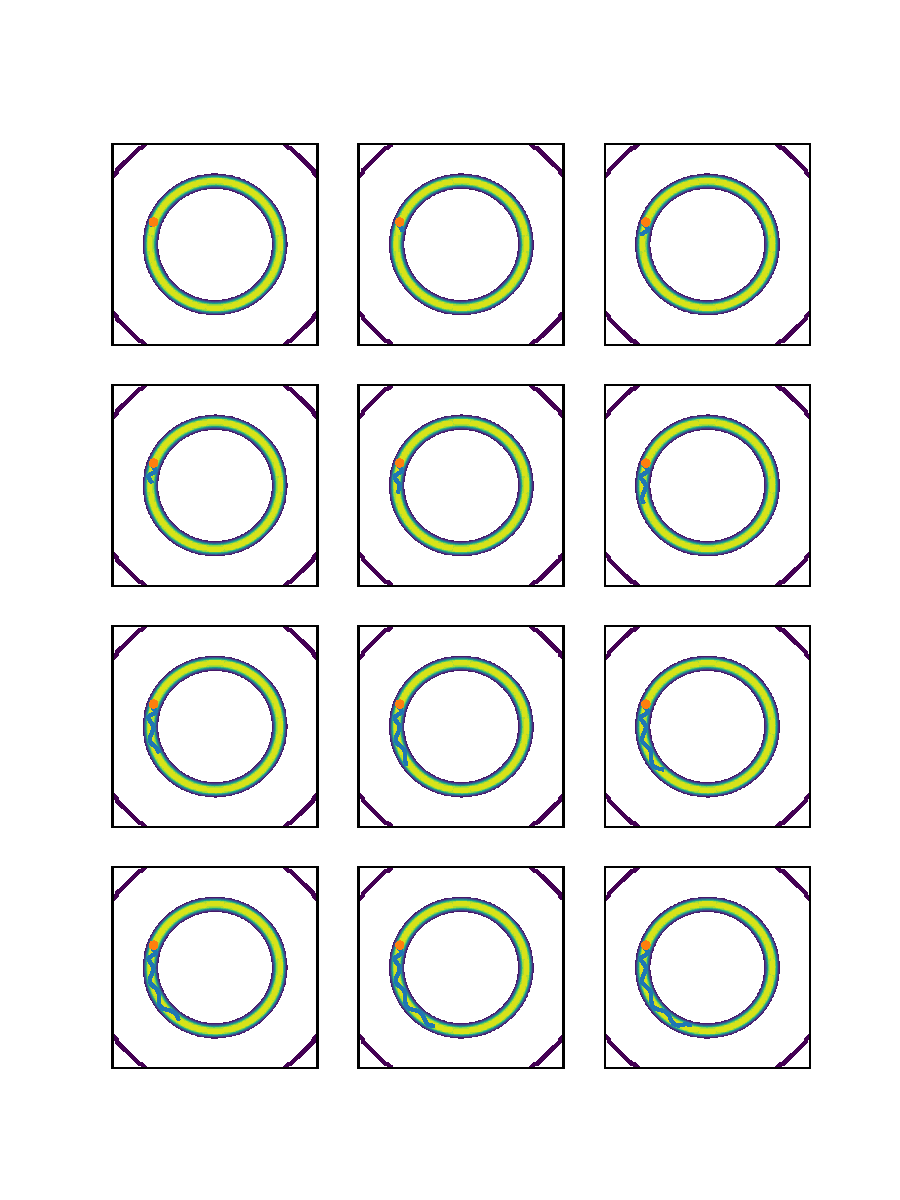
\includegraphics[width=\textwidth]{figures/hmc_trajectory}
  \caption{
    DP HMC proposal trajectory on a circular posterior
    (Section~\ref{circle_section}). The orange point is the starting
    point of the leapfrog simulation and the blue line shows the progress
    of the leapfrog steps. The background is a contour plot of the circular
    posterior density.
  }
  \label{hmc_trajectory_fig}
\end{figure}

\chapter{Experimental Setup}\label{experiment_setup_chapter}

To compare the performance of the DP MCMC algorithms, they were run on
several models. This chapter introduces these models in Sections~\ref{gauss_model},
\ref{banana_section} and \ref{circle_section}. The practicalities, such as
the hyperparameter values of the model and the initialisation of the
MCMC algorithms, are considered in Section~\ref{practical_section}.
Finally, the main performance
metric used in the experiments is introduced in Section~\ref{mmd_section}.
The results of the experiments are discussed in Chapter~\ref{experiment_chapter}.

\section{The Gaussian Model}\label{gauss_model}

The simplest model used for the experiments is the Gaussian model with
known covariance. The likelihood and prior for \(n\) points of \(d\)-dimensional
data \(X \in \R^{n\times d}\) and parameters \(\theta\in \R^{d}\) are
\begin{align*}
  \theta &\sim \caln_{d}(\mu_{0}, \Sigma_{0}), \\
  X_{i} &\sim \caln_{d}(\theta, \Sigma),
\end{align*}
where \(X_{i}\) is a row of \(X\), \(\Sigma\) is the known covariance,
and \(\mu_{0}\) and \(\Sigma_{0}\) are the prior hyperparameters.
The posterior of this model is another \(d\)-dimensional Gaussian distribution
with parameters expressible in closed form~\cite[Section 3.5]{BDA},
so it is easy to sample from the posterior.

\section{The Banana Distribution}\label{banana_section}

The banana distribution~\cite{TPK14} is a banana-shaped probability
distribution that is a challenging target for MCMC algorithms. For this reason it has
been used to test MCMC algorithms in the literature~\cite{TPK14}.

\begin{definition}
    Let \(X\) have a \(d\)-variate Gaussian distribution with
    mean \(\mu\) and covariance matrix \(\Sigma\). Let
    \[
        g(x) = (x_1, x_2 - a(x_1 - m)^2 - b, x_3, \dotsc, x_d),
    \]
    with \(a, b, m \in \R\).
    The banana distribution with parameters \(\mu, \Sigma, a, b\) and \(m\)
    is the distribution of \(g(X)\). It is denoted by
    \(\ban(\mu, \Sigma, a, b, m)\).
\end{definition}

In the literature, the banana distribution is simply used as the target to
sample from, and is not the posterior in a Bayesian inference
problem~\cite{TPK14}. To test differentially private MCMC algorithms, the
target distribution must be the posterior of some inference problem, as
otherwise there is no data to protect with differential privacy.
Theorem~\ref{banana_posterior_theorem} gives a suitable inference problem
for testing DP MCMC algorithms.

\begin{theorem}\label{banana_posterior_theorem}
    Let
    \begin{align*}
        \theta = (\theta_1,\dotsc, \theta_d) &\sim
        \ban(0, \sigma_0^2I, a, b, m), \\
        X_1 &\sim \caln(\theta_1, \sigma_1^2), \\
        X_2 &\sim \caln(\theta_2 + a(\theta_1 - m)^2 + b, \sigma_2^2),\\
        X_3 &\sim \caln(\theta_3, \sigma_3^2), \\
            &\vdots \\
        X_d &\sim \caln(\theta_d, \sigma_d^2). \\
    \end{align*}
    Given data \(x_1,\dotsc, x_d\in \R^n\) and
    denoting \(\tau_i = \frac{1}{\sigma_i^2}\),
    the posterior of \(\theta\) tempered with \(T\) is the banana distribution
    \(\ban(\mu, \Sigma, a, b, m)\)
    with
    \[
        \bar{x}_i = \frac{1}{n}\sum_{j=1}^n x_{ji} \quad i\in \{1, 2\}.
    \]
    \[
        \mu = \left(\frac{Tn\tau_1\bar{x}_1}{Tn\tau_1 + \tau_0},\dotsc,
        \frac{Tn\tau_d\bar{x}_d}{Tn\tau_d + \tau_0}\right),
    \]
    \[
        \Sigma = \diag\left(
            \frac{1}{Tn\tau_1 + \tau_0},\dotsc,
            \frac{1}{Tn\tau_d + \tau_0}
        \right).
    \]
\end{theorem}
\begin{proof}
  See Appendix~\ref{banana_posterior_theorem_proof}.
\end{proof}
\newcounter{banana_posterior_theorem_number}
\setcounter{banana_posterior_theorem_number}{\value{theorem}}

The Gaussian distribution is a special case of the banana distribution,
as setting \(a = 0\) makes \(g\) the identity function. Similarly, setting
\(a = 0\) turns the Bayesian banana model into a Gaussian model.


\section{Circle Model}\label{circle_section}

Random walk MH algorithms may struggle with posteriors which are concentrated
on long, but thin regions. Having a large proposal variance causes the algorithm
to frequently jump out of the region of high probability, but lowering the
variance to stay in the region causes the chain to take a very long time to move
around in the region. An example of such a posterior is the circular posterior
described in this section.

The circle posterior is obtained from a model where the log-likelihood is
\[
    \ln p(r\mid x, y) = -a(x^2 + y^2 - r^2)^2
\]
where \(r\in \R\) is an observed data point and \((x, y)\in \R^{2}\) are the
parameters.
The likelihood is circular in the \((x, y)\)-plane, as it only depends on the
squared distance of the point \((x, y)\) from the origin. By choosing a flat
prior, \(p(x, y) = 1\) for all \((x, y)\in \R^{2}\), the posterior will be
proportional to the likelihood, meaning that the posterior will also be circular.

As the prior does not integrate to 1, it is not a proper probability density,
so Bayes' theorem does not guarantee that the posterior integrates to a finite
value. In this case, for a single data point \(r\),
\begin{align*}
  \int_{\R^{2}}p(r\mid x, y)\dx x\dx y
  &= \int_{\R^{2}}e^{-a(x^{2} + y^{2} - r^{2})^{2}}\dx x\dx y
  \\&= \int_{0}^{2\pi}\dx \phi \int_{0}^{\infty}\dx t
  \cdot te^{-a(t^{2}(\cos^{2} \phi + \sin^{2} \phi) - r^{2})^{2}}
  \\&= \int_{0}^{2\pi}\dx \phi \int_{0}^{\infty}\dx t
  \cdot te^{-a(t^{2} - r^{2})^{2}}
  \\&= \int_{0}^{2\pi}\dx \phi \int_{0}^{\infty}\dx u\cdot e^{-a(u - r^{2})^{2}}
  \\&< \infty.
\end{align*}
As the inner integral is over an unnormalised Gaussian density and
the outer integral is over a finite interval. For multiple data points, the
integral of the likelihood is
\[
  \int_{\R^{2}}\prod_{i}^{n}p(r_{i}\mid x,y)\dx x\dx y
  \leq \prod_{i}^{n}\left(\int_{\R^{2}}p(r_{i}\mid x,y)^{n}\dx x\dx y\right)^{\frac{1}{n}}
  < \infty,
\]
where the first inequality is Hölder's inequality applied \(n - 1\) times,
and the second follows from the single data point case, as
\(p(r\mid x,y)^{n} = e^{-an(x^{2} + y^{2} - r^{2})^{2}}\).
As the likelihood integrates to a
finite value, it can be considered an unnormalised density and sampled from
with MCMC.

Obtaining samples from the true posterior with the circle model is not
as easy as with the banana and Gaussian models, so using MMD, the metric
introduced in Section~\ref{mmd_section} to evaluate
the performance of an MCMC algorithm on the circle is nontrivial. However,
as the mean of the circle is in its center, and the samples from an MCMC
algorithm are likely to lie on the circle, the distance of the mean of the
sample from the origin indicates how evenly the samples a distributed throughout
the circle.

It remains to show that the mean of the circle is actually the origin. It turns
out that this is fairly simple. For the mean of the \(x\)-coordinate
\begin{align*}
  E_{x} &= \int_{\R}\dx x\cdot x\int_{\R} \dx y p(r\mid x, y)
  \\&= \int_{-\infty}^{\infty}\dx x\cdot x\int_{-\infty}^{\infty}\dx y
  \prod_{i} e^{-a(x^{2} + y^{2} - r_{i}^{2})^{2}}
  \\&= \int_{0}^{\infty}\dx x\cdot x\int_{-\infty}^{\infty}\dx y
  \prod_{i} e^{-a(x^{2} + y^{2} - r_{i}^{2})^{2}}
  + \int_{-\infty}^{0}\dx x\cdot x\int_{-\infty}^{\infty}\dx y
  \prod_{i} e^{-a(x^{2} + y^{2} - r_{i}^{2})^{2}}
  \\&= \int_{0}^{\infty}\dx x\cdot x\int_{-\infty}^{\infty}\dx y
  \prod_{i} e^{-a(x^{2} + y^{2} - r_{i}^{2})^{2}}
  - \int_{0}^{\infty}\dx x\cdot x\int_{-\infty}^{\infty}\dx y
  \prod_{i} e^{-a(x^{2} + y^{2} - r_{i}^{2})^{2}}
  \\&= 0.
\end{align*}
The mean of the \(y\)-coordinate is calculated similarly.

Unlike the banana and Gaussian models,
the circle model does not give a method to generate the data points
\(r_{i}\) from given values of \(x\) and \(y\). The \(r_{i}\) values used
in the experiments of Chapter~\ref{experiment_chapter} were sampled
from a normal distribution with mean 3 and variance 1.

\section{Practicalities of Running the MCMC Algorithms}\label{practical_section}

Eight sets of model hyperparameters were used in the experiments.
The hyperparameters are shown in
Table~\ref{model_params_table} and contour plots of the
2-dimensional models are shown in Figure~\ref{posterior_plots_fig}.
All banana models had \(b = m = 0\). The likelihood variance of the banana
and 30-dimensional Gaussian
models was \(\sigma_{1}^{2} = 20\), \(\sigma_{2}^{2} = 2.5\) and
\(\sigma_{i}^{2} = 1\)
for \(i > 2\). The likelihood covariance for the correlated Gaussian model
was
\[
\begin{bmatrix}
  1 & 0.999 \\
  0.999 & 1
\end{bmatrix}.
\]
The true values of \(\theta\) in all experiment except the circle are
\(\theta_{2} = 3\) and \(\theta_{i} = 0\) for \(i \neq 2\).


All experiments ran 20 chains for each value
of \(\epsilon\) for DP MCMC experiments, or clip bound for clipping experiments,
for each algorithm included. Each of the
20 chains had a different starting point, chosen from a Gaussian
distribution value with standard deviation as
shown in Table~\ref{model_params_table}, but the starting points did
not vary across algorithms, or values of \(\epsilon\) or clip bound.
The Gaussian distribution choosing the starting points was
centered on the true parameter values for the banana and Gaussian experiments,
and on \((0, 1)\) for the circle experiment.

The first half of the obtained samples were discarded as they may not represent
the true posterior, which is standard practice with MCMC~\cite{BDA}. The
latter half was compared to a reference sample obtained from the true posterior,
except in the circle experiment, where the mean of the sample was compared to
the true posterior mean of \((0,0)\).

Publicly available implementations of DP
Barker\footnote{\url{https://github.com/DPBayes/DP-MCMC-NeurIPS2019}}
and the Fourier
accountant\footnote{\url{https://github.com/DPBayes/PLD-Accountant}} were
used, and the rest of the algorithms were implemented by the author.
The accuracy and running time of the Fourier acountant is
determined by two parameters~\cite{KJH20}. They were left at their default values.
The code for running the experiments is freely
available\footnote{\url{https://github.com/oraisa/masters-thesis}}.

\begin{figure}[h]
  \centering
  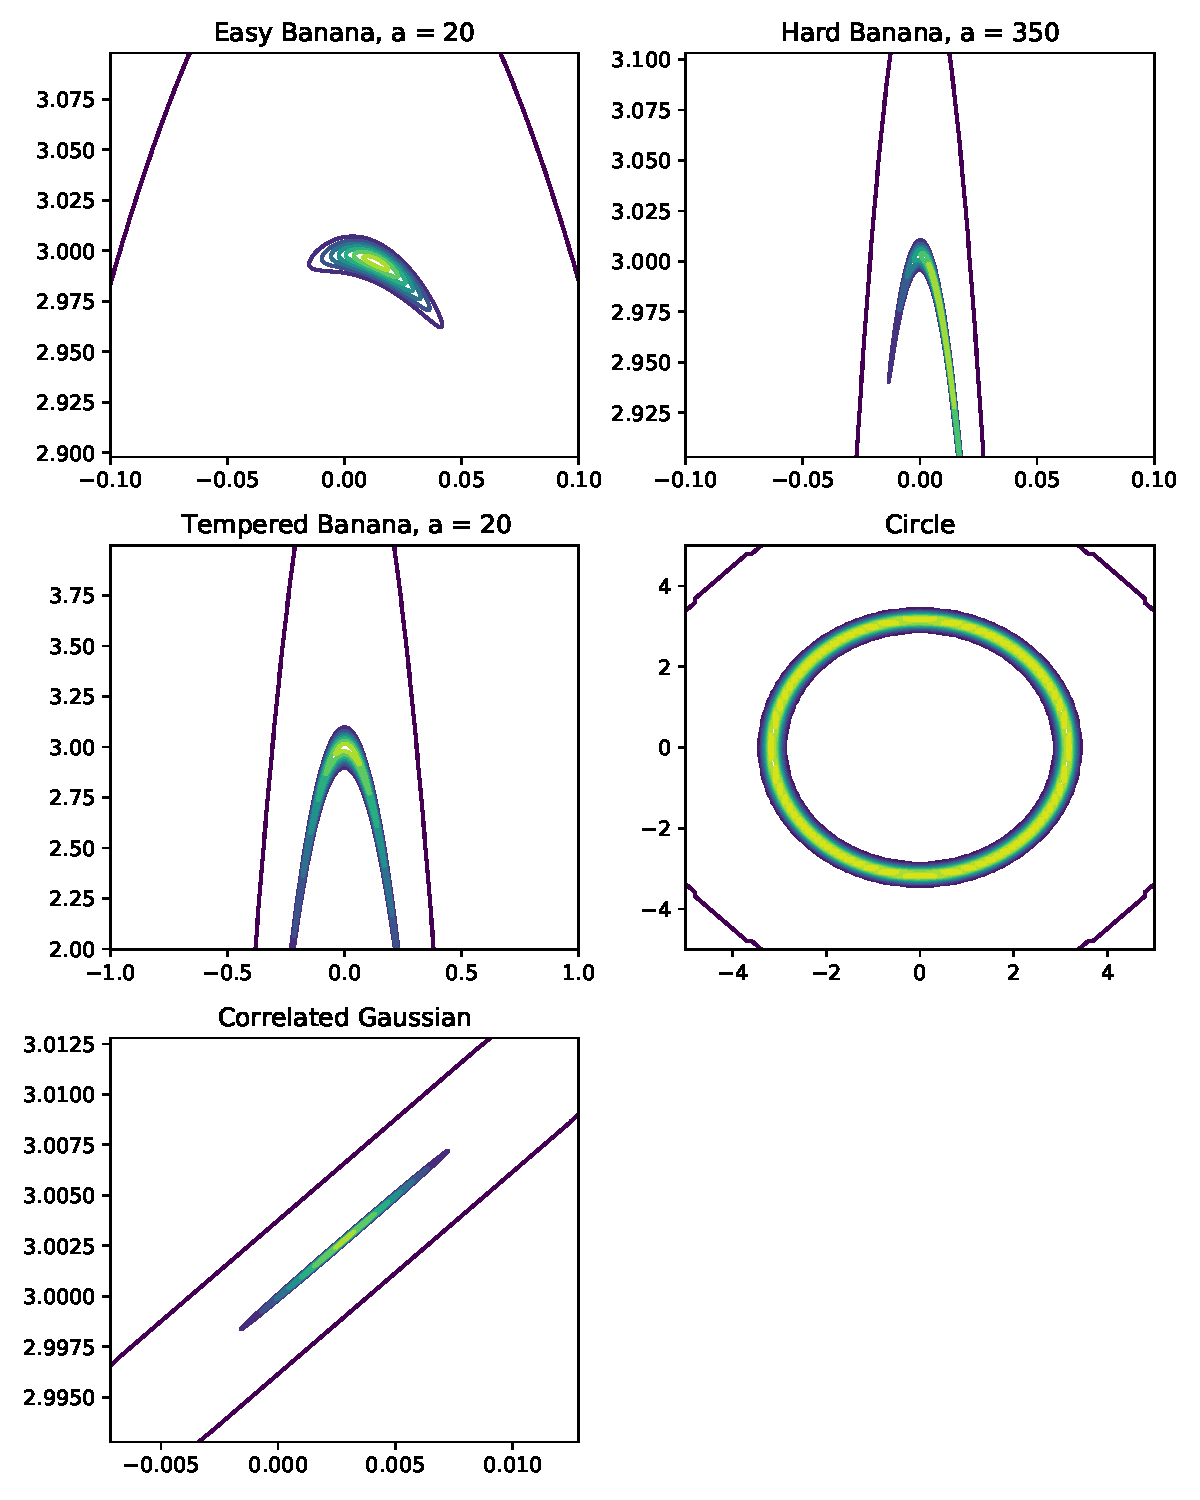
\includegraphics[width=\textwidth]{figures/posterior_plots}
  \caption{
    Contour plots of the posterior densities of the 2-dimensional models.
  }
  \label{posterior_plots_fig}
\end{figure}

\begin{table}[h]
\centering
\caption{
            Model hyperparameters. $n_0$ determines tempering by \(T=\frac{n_0}{n}\).
            For missing $n_0$, \(T = 1\).
            }
\label{model_params_table}
\begin{tabular}{lrrrrr}
\toprule
                   Name &  d &      n &  $n_0$ &     a &  $\sigma^2_0$ \\
\midrule
     Flat banana, d = 2 &  2 & 100000 &        &    20 &          1000 \\
    Flat banana, d = 10 & 10 & 200000 &        &    20 &          1000 \\
 Tempered banana, d = 2 &  2 & 100000 &   1000 &    20 &          1000 \\
Tempered banana, d = 10 & 10 & 200000 &   1000 &    20 &          1000 \\
 High dimensional Gauss & 30 & 200000 &        &     0 &          1000 \\
          Narrow banana &  2 & 150000 &        &   350 &          1000 \\
       Correlated Gauss &  2 & 200000 &        &     0 &           100 \\
                 Circle &  2 & 100000 &        & 1e-05 &               \\
\bottomrule
\end{tabular}
\end{table}


\section{Maximum Mean Discrepancy}\label{mmd_section}

The convergence of non-DP MCMC algorithms is typically assessed using 
\(\hat{R}\)~\cite{BDA}, which measures how well multiple chains started from 
different points have mixed together. The utility of a sample produced by an 
MCMC algorithm can be evaluated using effective sample size (ESS)~\cite{BDA},
which is an estimate of the size of an uncorrelated sample of the posterior
with the same estimation utility as the MCMC sample. 

Both \(\hat{R}\) and ESS require that the MCMC algorithm asymptotically targets 
the true posterior, as they cannot detect an algorithm that has converged to the 
wrong distribution. Because some of the DP MCMC algorithms use approximations 
that may cause the algorithms to not converge to the true posterior, 
such as clipping the log-likelihood ratios, \(\hat{R}\) and ESS are not suitable
for assessing the performance of the algorithms.

Because the DP MCMC algorithms may not converge to the correct distribution, 
their performance should be evaluated with a metric that measures how close 
to the true distribution they are. A very general such metric is maximum mean
discrepancy (MMD)~\cite{GrettonBRSS12}. MMD between distributions \(p\) and \(q\) 
is defined as 
\[
    \mathrm{MMD}(p, q) = \sup_{f\in \mathcal{F}}(E_{x\sim p}f(x) - E_{y\sim q}f(y))
\]
where \(\mathcal{F}\) is some class of functions. By 
choosing a suitable \(\mathcal{F}\), \(\mathrm{MMD}(p, q)\) can be estimated from a 
sample from \(p\) and \(q\). The suitable classes \(\mathcal{F}\) can be 
characterised by a kernel function \(k\colon P\times Q \to \R\), where 
\(P\) and \(Q\) are the supports of \(p\) and \(q\), respectively.
The Gaussian radial basis function (RBF) kernel 
\[
    k(x, y) = \exp\left(\frac{||x - y||_2^2}{2\sigma^2}\right)
\]
is particularly well suited, as it has the property that 
\(\mathrm{MMD}(p, q) = 0\) if and only if \(p = q\). After choosing a kernel,
\(\mathrm{MMD}(p, q)\) may be estimated from finite samples of \(p\) and \(q\).
To evaluate MCMC algorithms, one of the samples is the output of the algorithm 
to be evaluated, and the other is a sample from the true posterior.

The choice of the \(\sigma\) parameter of \(k\) affects the way MMD evaluates 
different kinds of differences in \(p\) and \(q\). For some preliminary experiments
in this thesis, \(\sigma\) was chosen to be 1, which penalised error in the 
mean much more than errors in higher moments in the experiments. 
The \(\sigma\) used for the final experiments is chosen by picking 50 subsamples
from both samples with replacement and setting \(\sigma\) to be the median 
between distances of points of the subsamples. This is following the procedure of 
Gretton et al.~\cite{GrettonBRSS12}, with the addition of the subsampling step
to handle samples of different sizes.

\chapter{Experiments}\label{experiment_chapter}

This chapter contains the experiments performed on both non-DP and DP MCMC
algorithms. Section~\ref{accounting_comparison_section} compares the
zCDP, RDP and ADP based privacy accounting methods that are available
for DP penalty, minibatch DP Penalty and DP HMC.
Section~\ref{clipping_experiments}
examines the effect clipping log-likelihood ratios, which is necessary for
DP MCMC algorithms, but may adversely affect their convergence.
Section~\ref{dp_mcmc_comparison} compares the different DP MCMC algorithms
on several models.

\section{Comparing Privacy Accounting Methods}\label{accounting_comparison_section}

DP penalty, minibatch DP penalty and DP HMC have two different methods to
compute the number of iterations the algorithm can run for, given a privacy
bound and parameters for the algorithm. These privacy accounting methods
are given by Theorems~\ref{DP_penalty_theorem_zcdp} and
\ref{DP_penalty_theorem_adp} for DP penalty, Theorems~\ref{dp_hmc_theorem_zcdp}
and \ref{dp_hmc_theorem_adp} for DP HMC, and
Theorem~\ref{dp_penalty_minibatch_theorem} and the Fourier
accountant~\cite{KJH20} for minibatch DP penalty.

Figure~\ref{accounting_comparison_fig} compares the number of iterations
each of the algorithms can run for for both accounting methods and different
values of \(\epsilon\) in the 2-dimensional flat banana experiment.
The ADP based methods of Theorems~\ref{DP_penalty_theorem_adp}
and \ref{dp_hmc_theorem_adp}, as well as the Fourier accountant, significantly
outperform the other accounting methods. This makes it clear that the tight
bounds given by the ADP based methods should be used in favor of loose methods.
The Fourier accountant is not easily applicable to DP Barker, as DP Barker
does not release the sample variance directly, it may still be possible
to use the Fourier accountant with DP Barker. This is an interesting question
for future research, as using a better privacy accountant may significantly
improve the performance of DP Barker.

\begin{figure}[h]
	\centering
  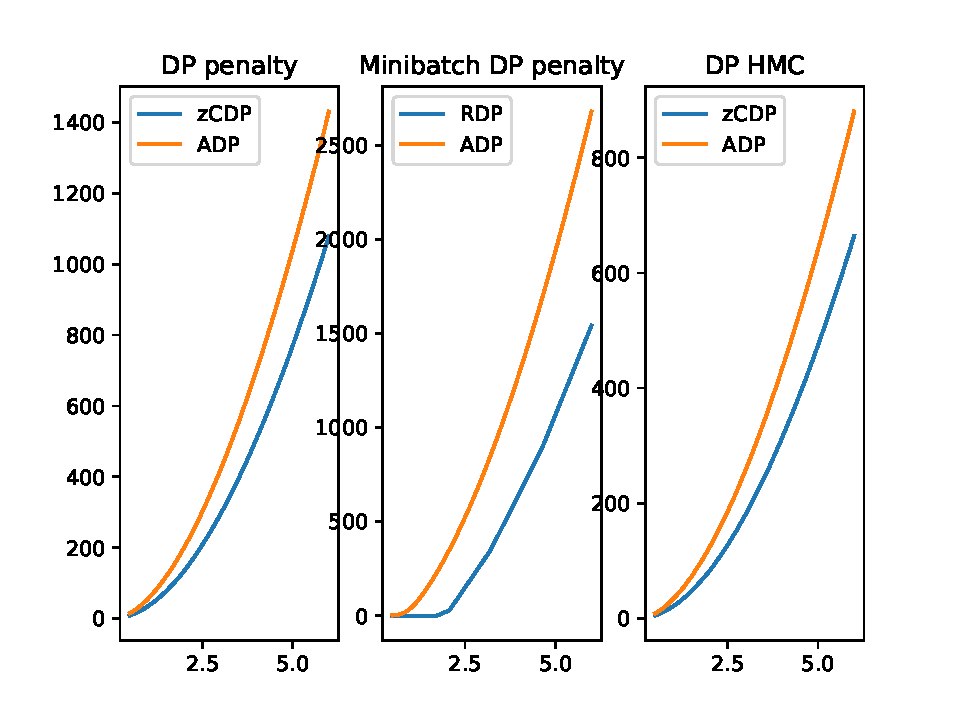
\includegraphics[width=\textwidth]{figures/accountant_comparison}
  \caption{
    Comparing the zCDP or RDP and ADP based privacy accounting methods
    for the algorithms with multiple accounting methods. The left panel
    compares zCDP based accounting (Theorem~\ref{DP_penalty_theorem_zcdp})
    and ADP based accounting (Theorem~\ref{DP_penalty_theorem_adp}) for
    the DP penalty algorithm. The middle panel compares the RDP accounting
    (Theorem~\ref{dp_penalty_minibatch_theorem}) and the Fourier accountant.
    The right panel compares the zCDP (Theorem~\ref{dp_hmc_theorem_zcdp})
    and ADP (Theorem~\ref{dp_hmc_theorem_adp}) based accounting.
    The ADP based methods significantly outperform the other methods
    in all cases.
  }
  \label{accounting_comparison_fig}
\end{figure}

\section{The Effects of Clipping}\label{clipping_experiments}

The first experiment evaluates the effect of clipping log-likelihood ratios.
Both HMC and random walk Metropolis-Hastings (RWMH)\footnote{Metropolis-Hastings using the Gaussian
distribution as the proposal distributions.}
algorithms were run on 2 and 10 dimensional banana models.
DP was not used so that error from the extra noise would not affect the results.

For both 2 and 10 dimensions, 500 samples from HMC and 3000 samples from
RWMH were taken and the latter half of them were
compared to 2000 samples from the true posterior. The reference posterior sample 
was also compared to other samples from the posterior to obtain a baseline.
The sample sizes and other parameters of the algorithms were tuned so that
the algorithms converged without clipping.

Figure~\ref{clip_effect_fig} shows the results of the clipping experiment.
The top left and bottom left panels show MMD as a function of the clip bound 
and the fraction of log-likelihoods that was actually clipped for both
HMC and RWMH in the 2-dimensional model. The effect of clipping on MMD 
is nonexistent for all but the lowest clip bounds. The top and bottom right 
panels show results for the 10-dimensional model. This time there are chains 
that did not converge correctly with most clip bounds, but the chains with 
the higher bounds converged. Based on these results, if the clip fraction is 
less than 10\%, clipping is likely undetectable without a large sample.

\begin{figure}[h]
    \centering
    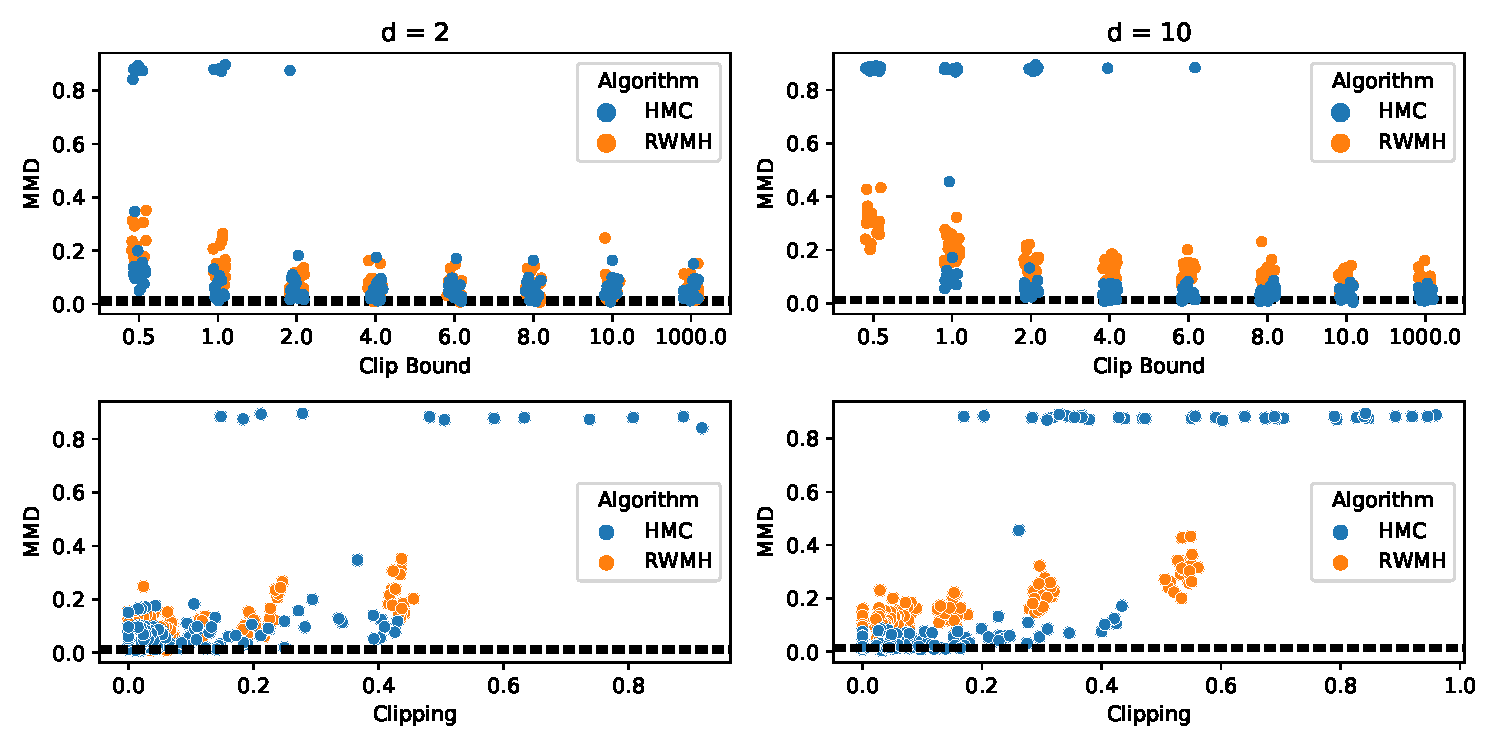
\includegraphics[width=\textwidth]{figures/clipping.pdf}
    \caption{
        The effect of log-likelihood ratio clipping on the posterior of the
        banana model for random walk Metropolis-Hastings and HMC.
        The top row shows posterior MMD as a function of the clip bound, and 
        the bottom row shows MMD as a function of the fraction of log-likelihoods
        that were clipped. The left columns used a 2-dimensional posterior 
        while the right columns had a 10-dimensional posterior. 
        The black lines show the MMDs of ten different samples of the true posterior
        compared to the reference sample. All of the lines are close the each 
        other and appear as a single line.
    }
    \label{clip_effect_fig}
\end{figure}

\section{Comparison of DP MCMC Algorithms}\label{dp_mcmc_comparison}

The experiments in this section compare the DP MCMC algorithms discussed in this
thesis. The compared algorithms are the DP penalty algorithm with and without
guided walk MH and one component updates~\cite{YildirimE19}
(Section~\ref{dp_penalty_section}), the DP Barker algorithm~\cite{HeikkilaJDH19}
(Section~\ref{dp_barker_section}), the penalty algorithm with subsampling, again
with and without GWMH and OCU (Section~\ref{dp_minibatch_penalty_section}) and
DP HMC (Section~\ref{dp_hmc_section}).

The \(\delta\) for all experiments is \(\frac{0.1}{n}\), and \(\epsilon\) is
varied.
All algorithms used the best privacy accounting methods discussed in this thesis.
For both variants of DP penalty and DP HMC, these are the PLD based
Theorems~\ref{DP_penalty_theorem_adp} and \ref{dp_hmc_theorem_adp}.
DP penalty with subsampling uses the Fourier accountant~\cite{KJH20}
and DP Barker uses Theorem~\ref{dp_barker_theorem}. The RDP based theorems
for the minibatch algorithms are not tight for the ADP bounds that were used,
so their results could be improved by using an accounting method for ADP.

The hyperparameters of the algorithms
were tuned by running the algorithms with \(\epsilon = 4\) and examining the
results, trying to find hyperparameters that minimise MMD. Clip bounds were
tuned so that less than 10\% of the log-likelihood ratios were clipped,
as the results of Section~\ref{clipping_experiments} show minimal effect on
MMD at that point.

Figure~\ref{banana_mmd_fig} shows the MMD for each algorithm as a function of
\(\epsilon\) for the flat and tempered banana models with 2 and 10 dimensions.
In the non-tempered models, the minibatch algorithms are not very useful,
with the exception of DP Barker in 10 dimensions. Of the non-minibatch algorithms,
with tempering HMC beats the penalty algorithms, but without tempering this is
reversed.

\begin{figure}
  \centering
  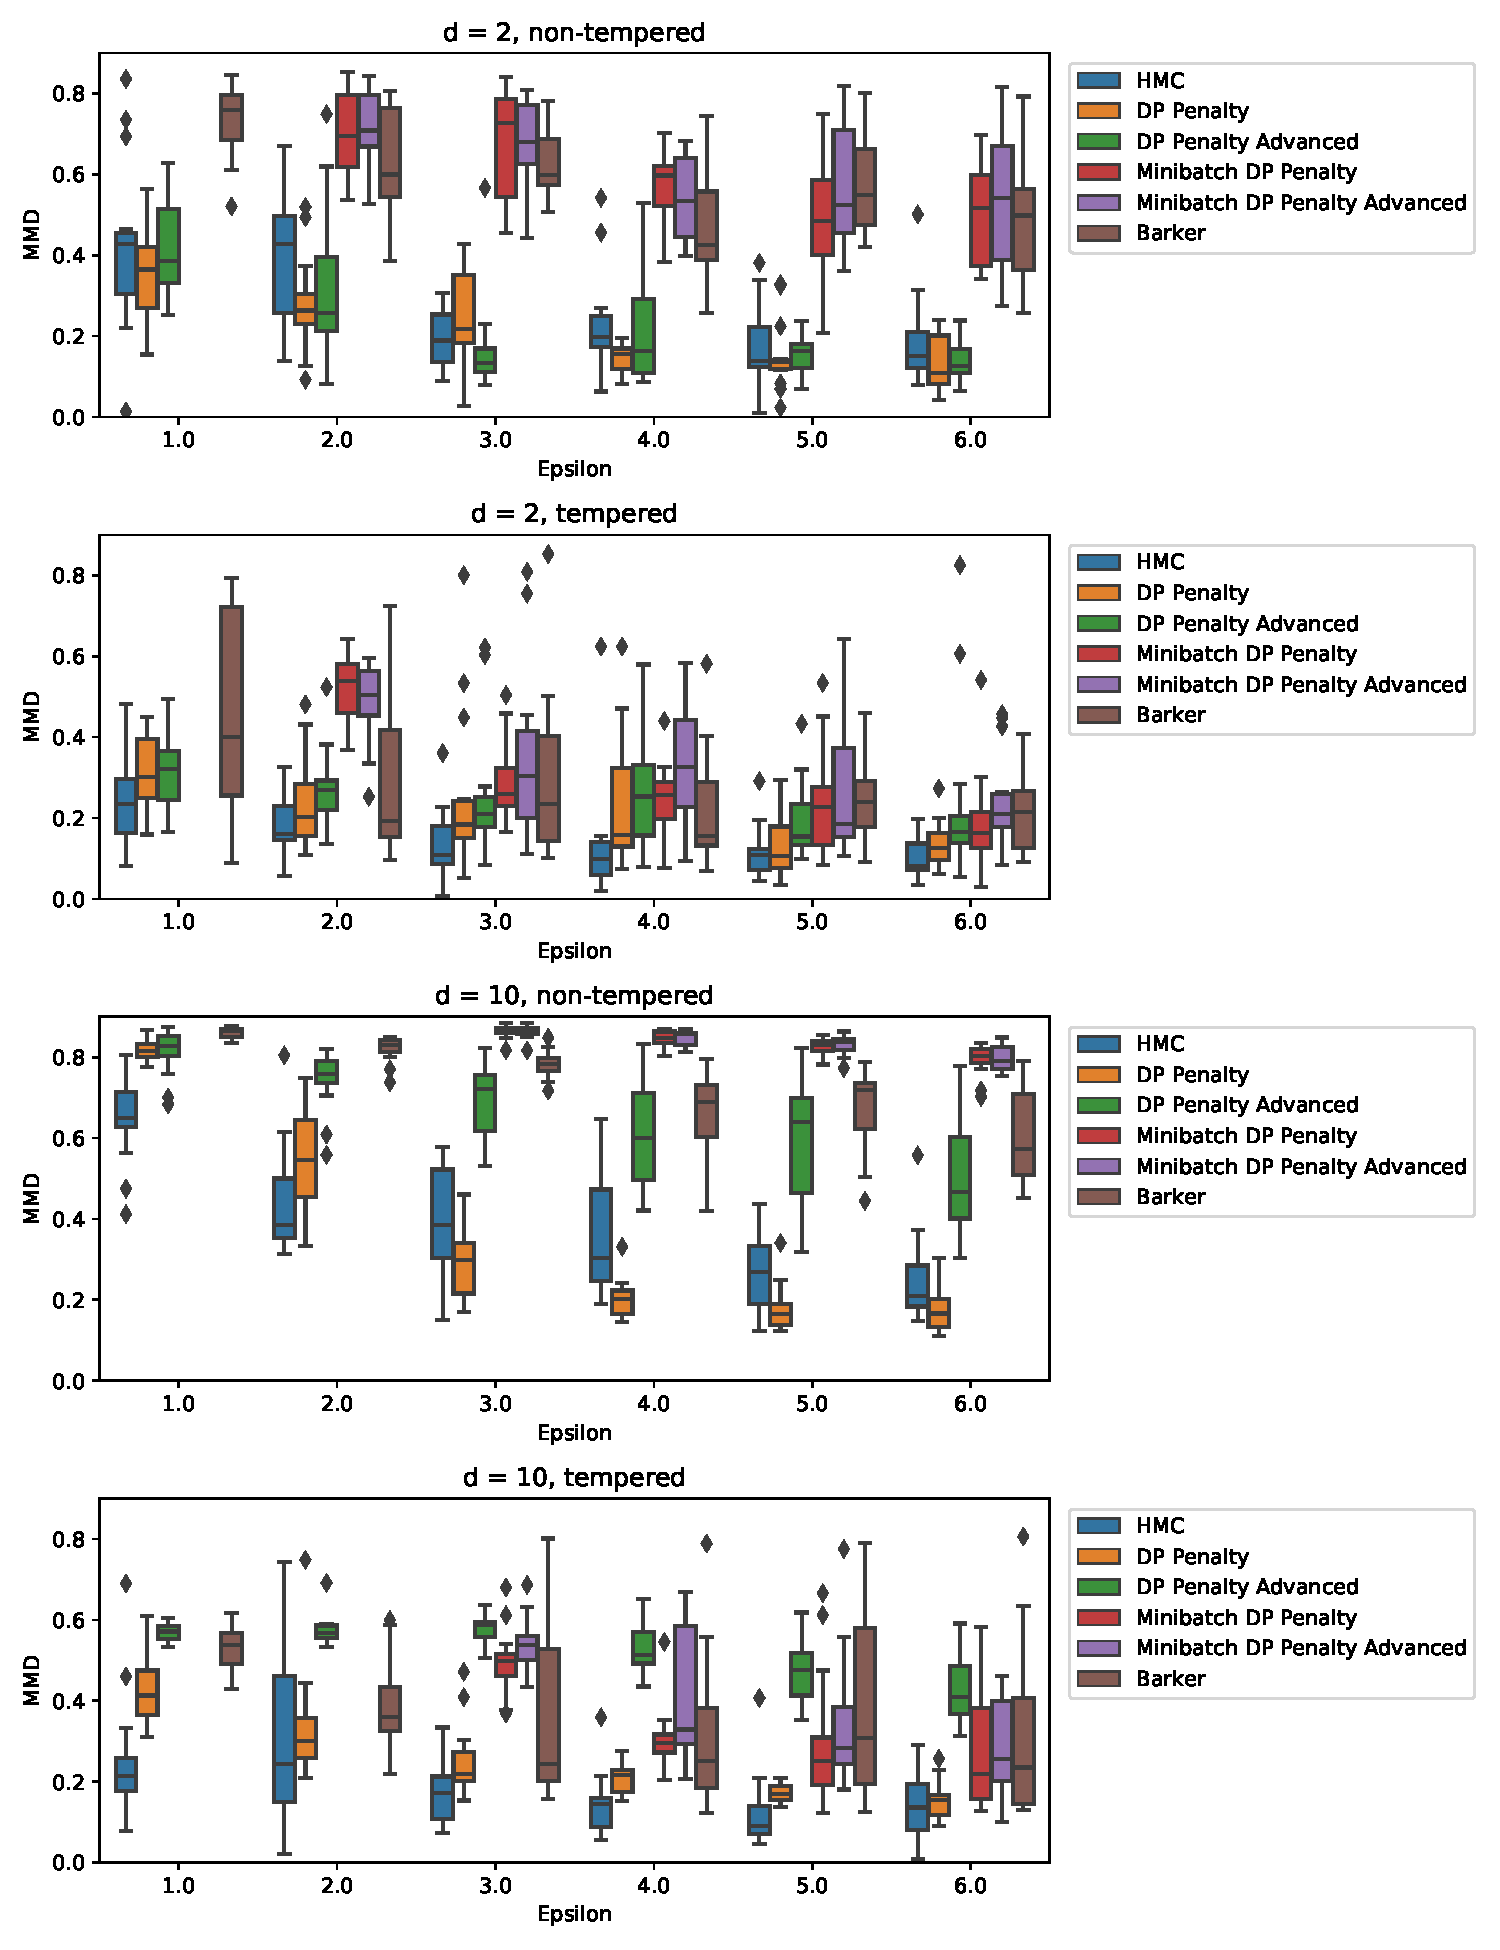
\includegraphics[width=\textwidth]{figures/banana_mmd.pdf}
  \caption{
    MMD as a function of \(\epsilon\) for the different MCMC algorithms,
    on flat and tempered banana models with both a low number of dimensions (2)
    and a high number of dimensions (10).
  }
  \label{banana_mmd_fig}

\end{figure}

Figure~\ref{banana_extra_mmd_fig} shows MMDs for the more complicated models,
the 30-dimensional Gaussian, the narrow banana and the highly correlated Gaussian.
The minibatch algorithms were not included as the previous experiment indicates
that they perform poorly without tempering.
In the 30-dimensional Gaussian, DP penalty with OCU and GWMH beats the other
two algorithms, with DP HMC narrowly beating DP penalty. In the narrow
banana all algorithms are approximately equal, until \(\epsilon = 4\) where
DP penalty0 OCU+GWMH has huge variance in MMD, and in the higher values of
\(\epsilon\) where it performs extremely poorly. In the highly correlated
Gaussian experiment, the penalty algorithms perform equally, and HMC beats
both of them.

\begin{figure}
  \centering
  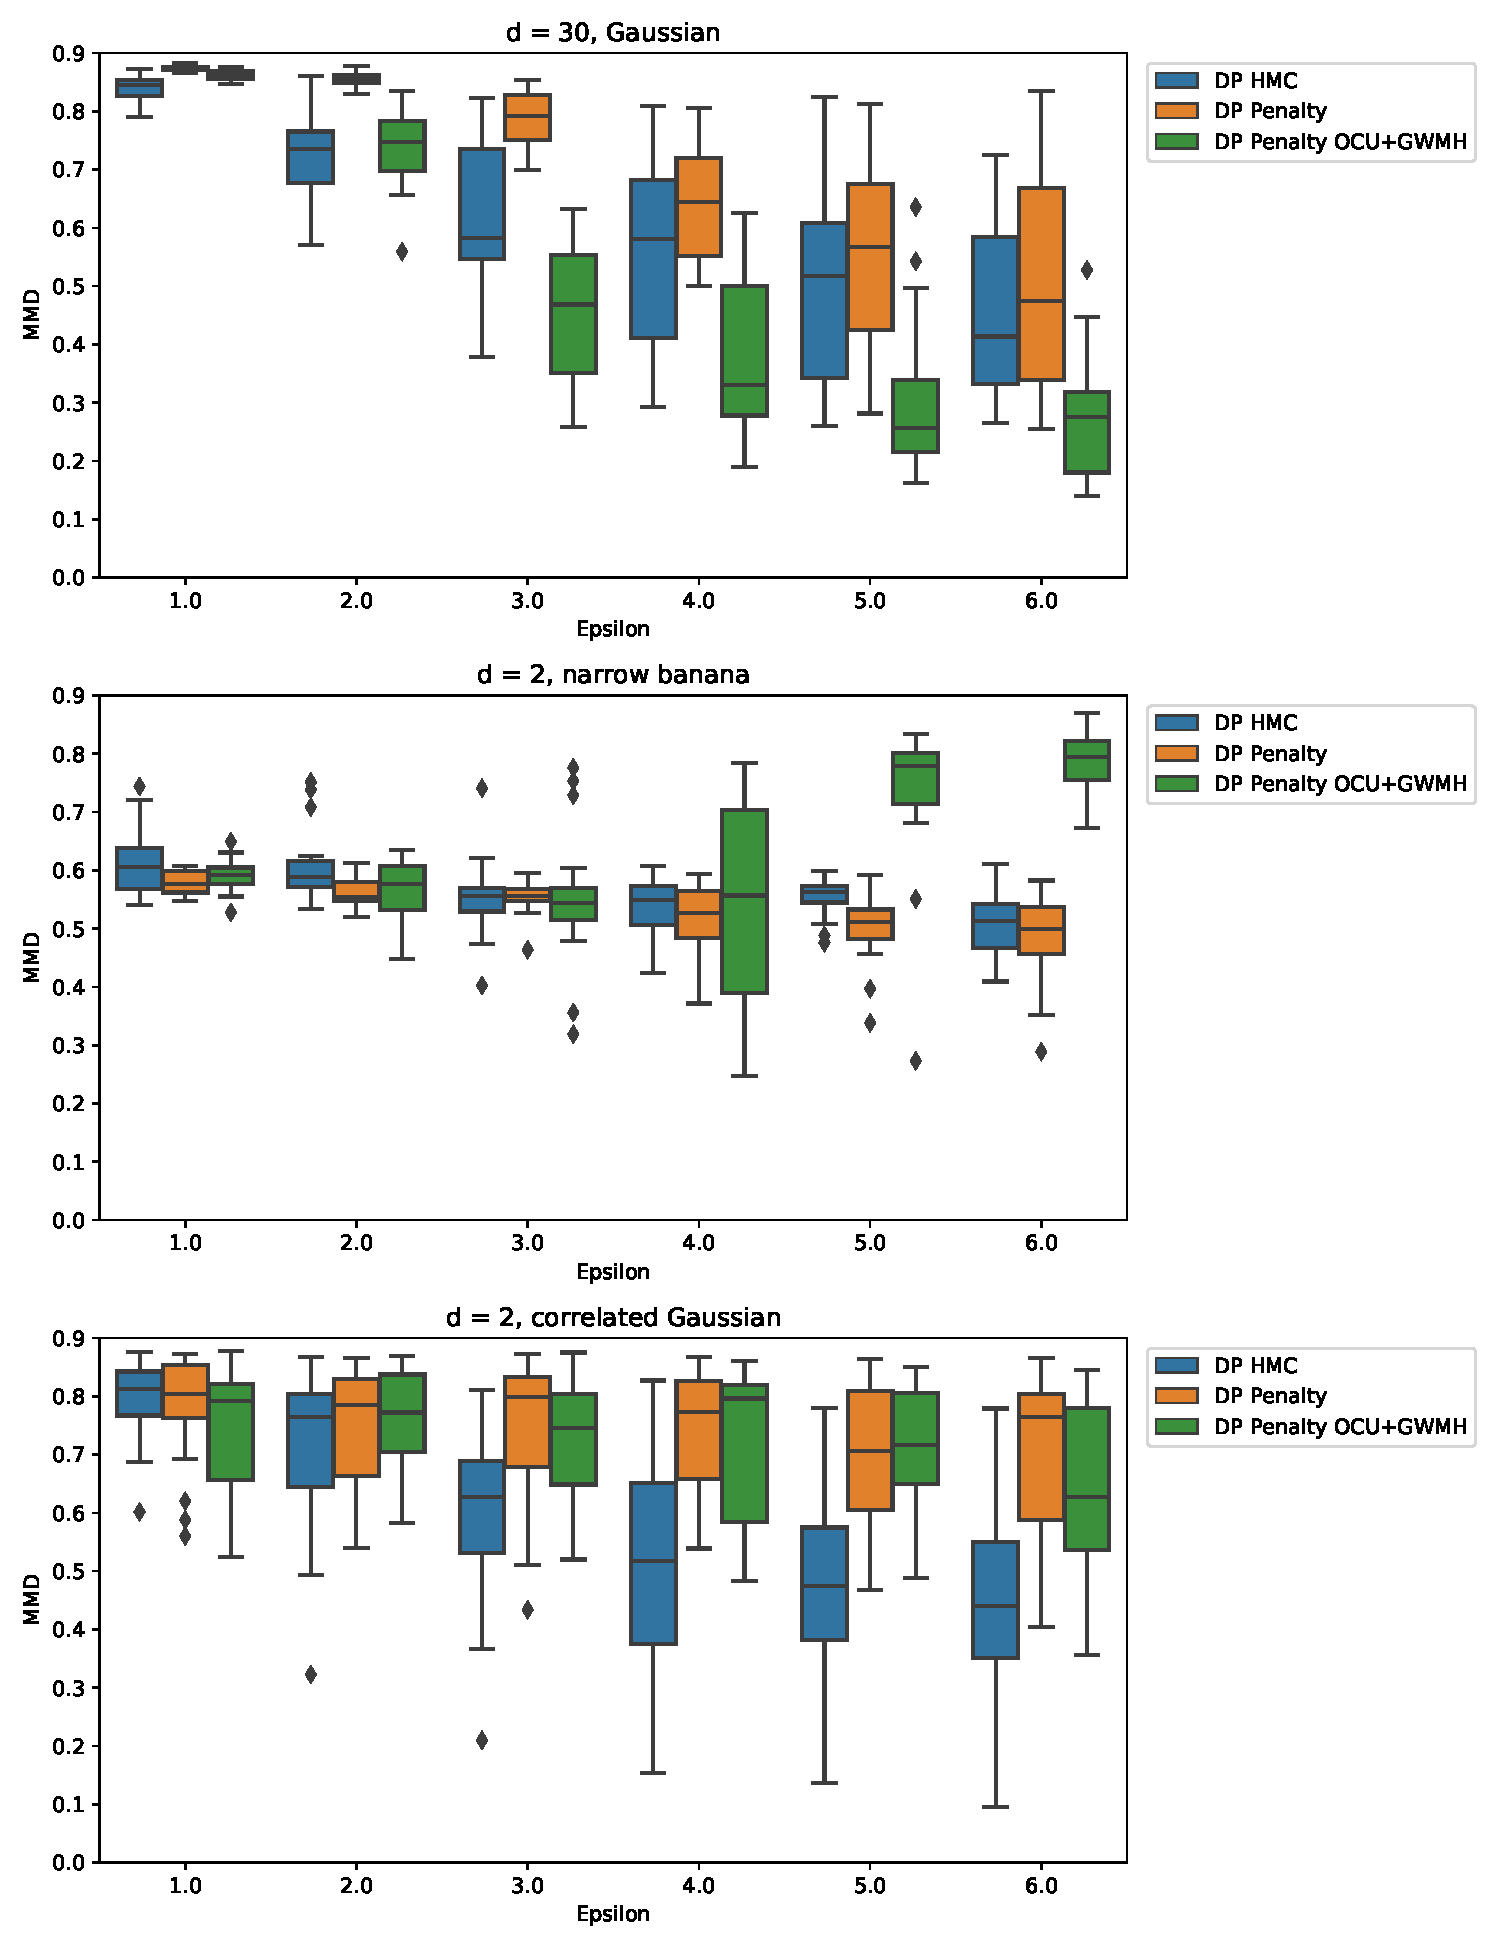
\includegraphics[width=\textwidth]{figures/banana_extra.pdf}
  \caption{
    MMD for the 30-dimensional Gaussian, hard banana and highly correlated
    2-dimensional Gaussian.
  }
  \label{banana_extra_mmd_fig}
\end{figure}

Figure~\ref{banana_clipping_fig} shows the fraction of log-likelihood ratios
that were clipped for each \(\epsilon\) and algorithm. Almost all runs had
less than 10\% clipping, with the exception of DP Barker, as adjusting its
clip bound is not possible.

\begin{figure}
  \centering
  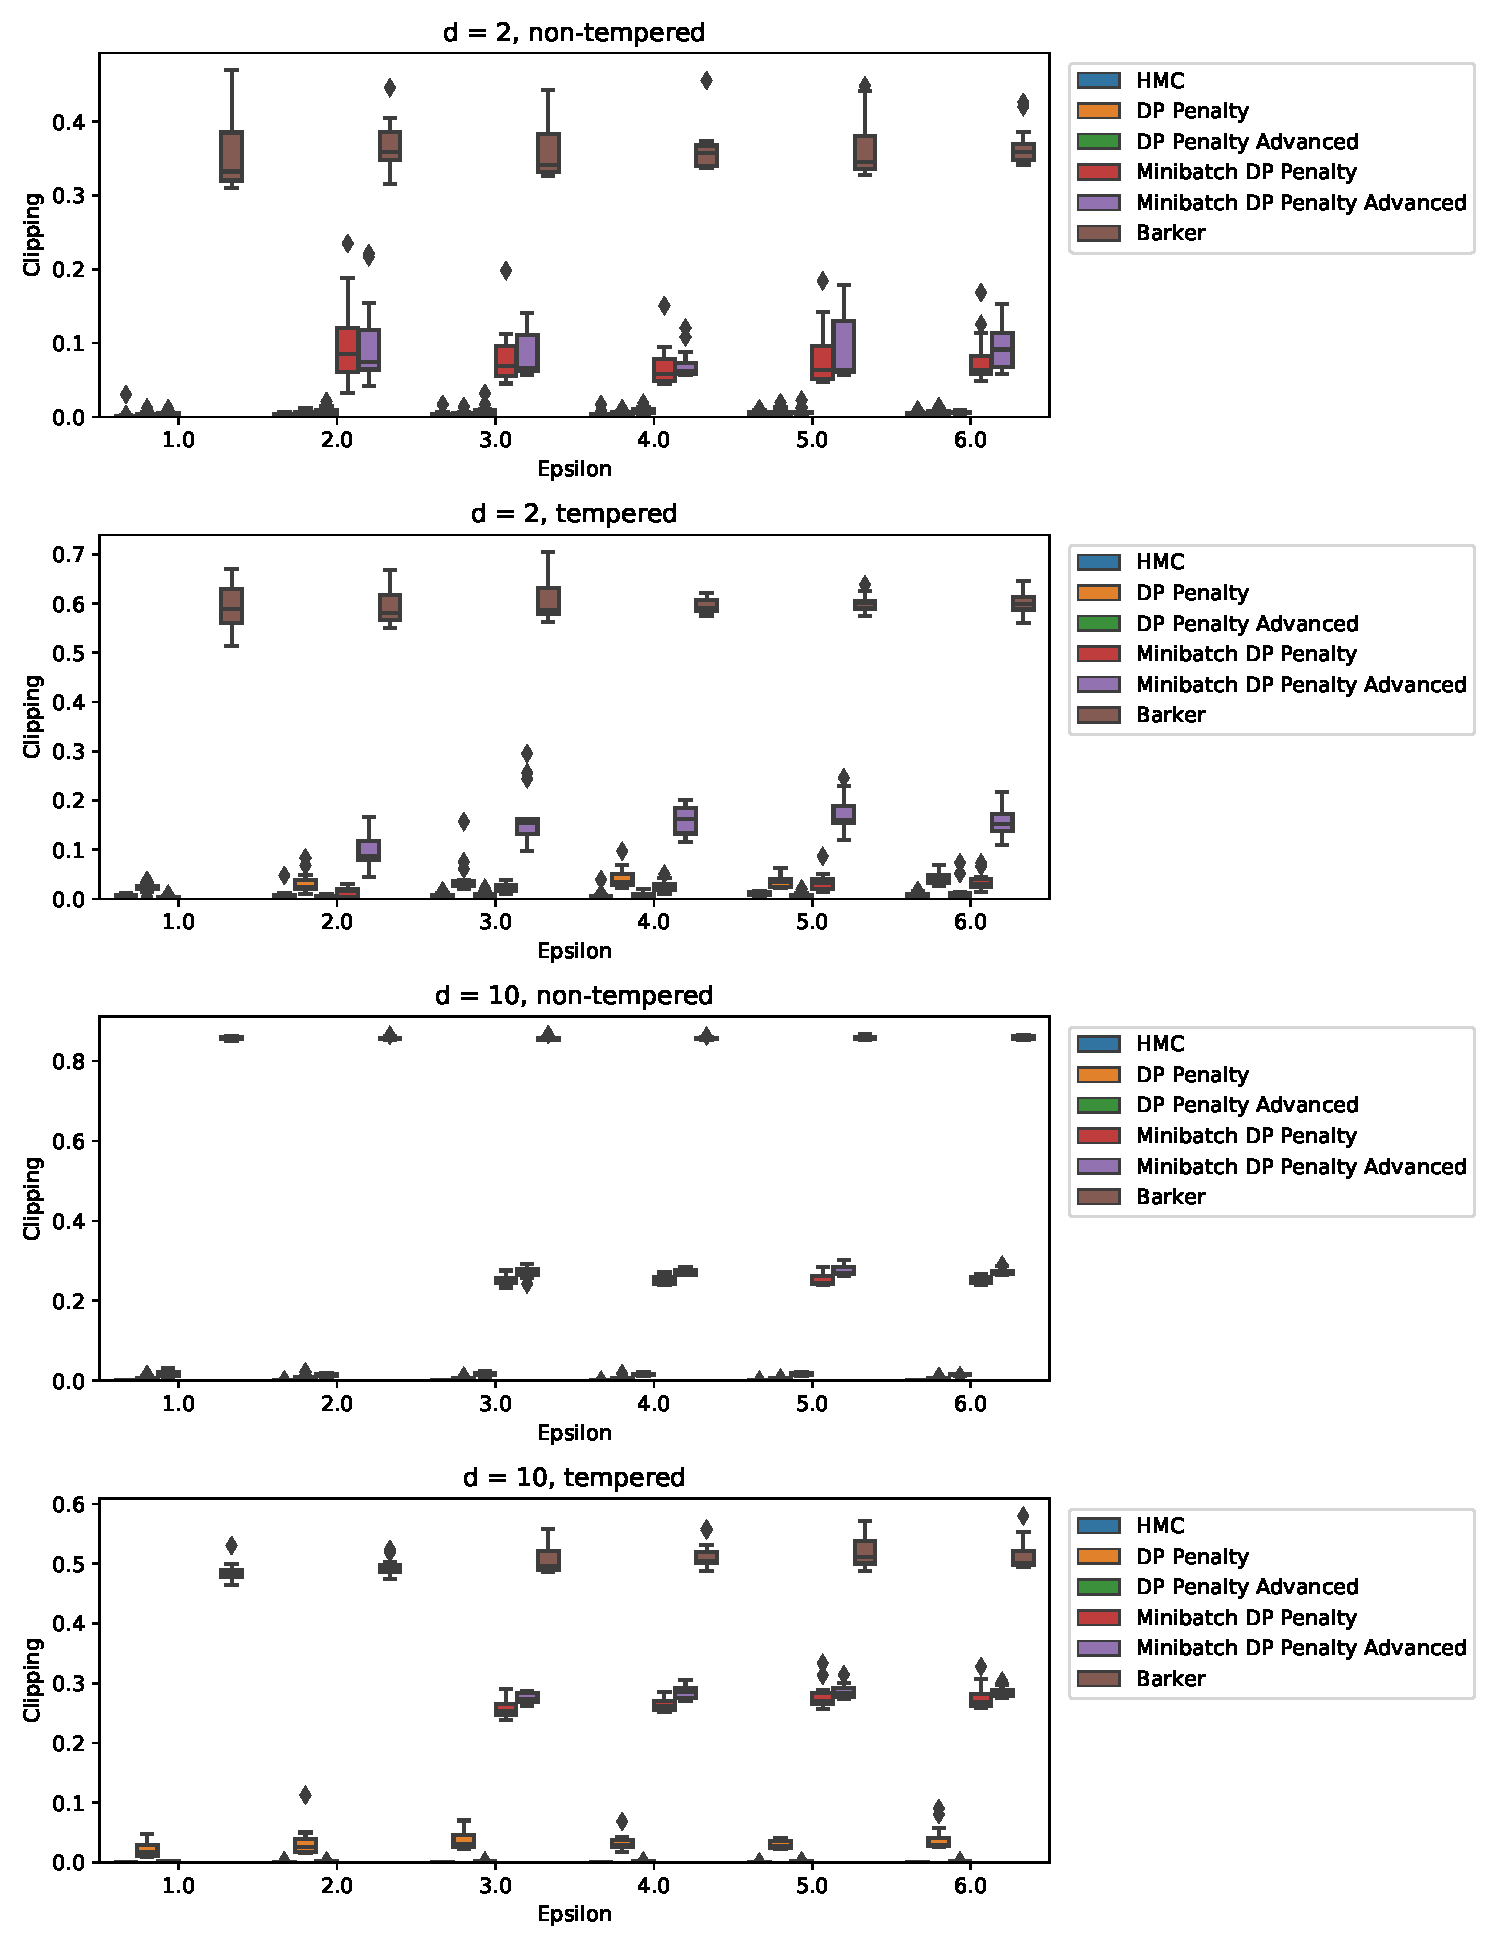
\includegraphics[width=\textwidth]{figures/banana_clipping.pdf}
  \caption{
    Clipping for the easy and tempered banana experiments.
  }
  \label{banana_clipping_fig}
\end{figure}

Figure~\ref{banana_extra_clipping_fig} shows clipping for the harder models.
Again, almost all runs have less than 10\% clipping, with the exception of
DP penalty OCU+GWMH on the narrow banana, where the high amount of clipping
could explain the poor performance of the algorithm with larger values
of \(\epsilon\).

\begin{figure}
  \centering
  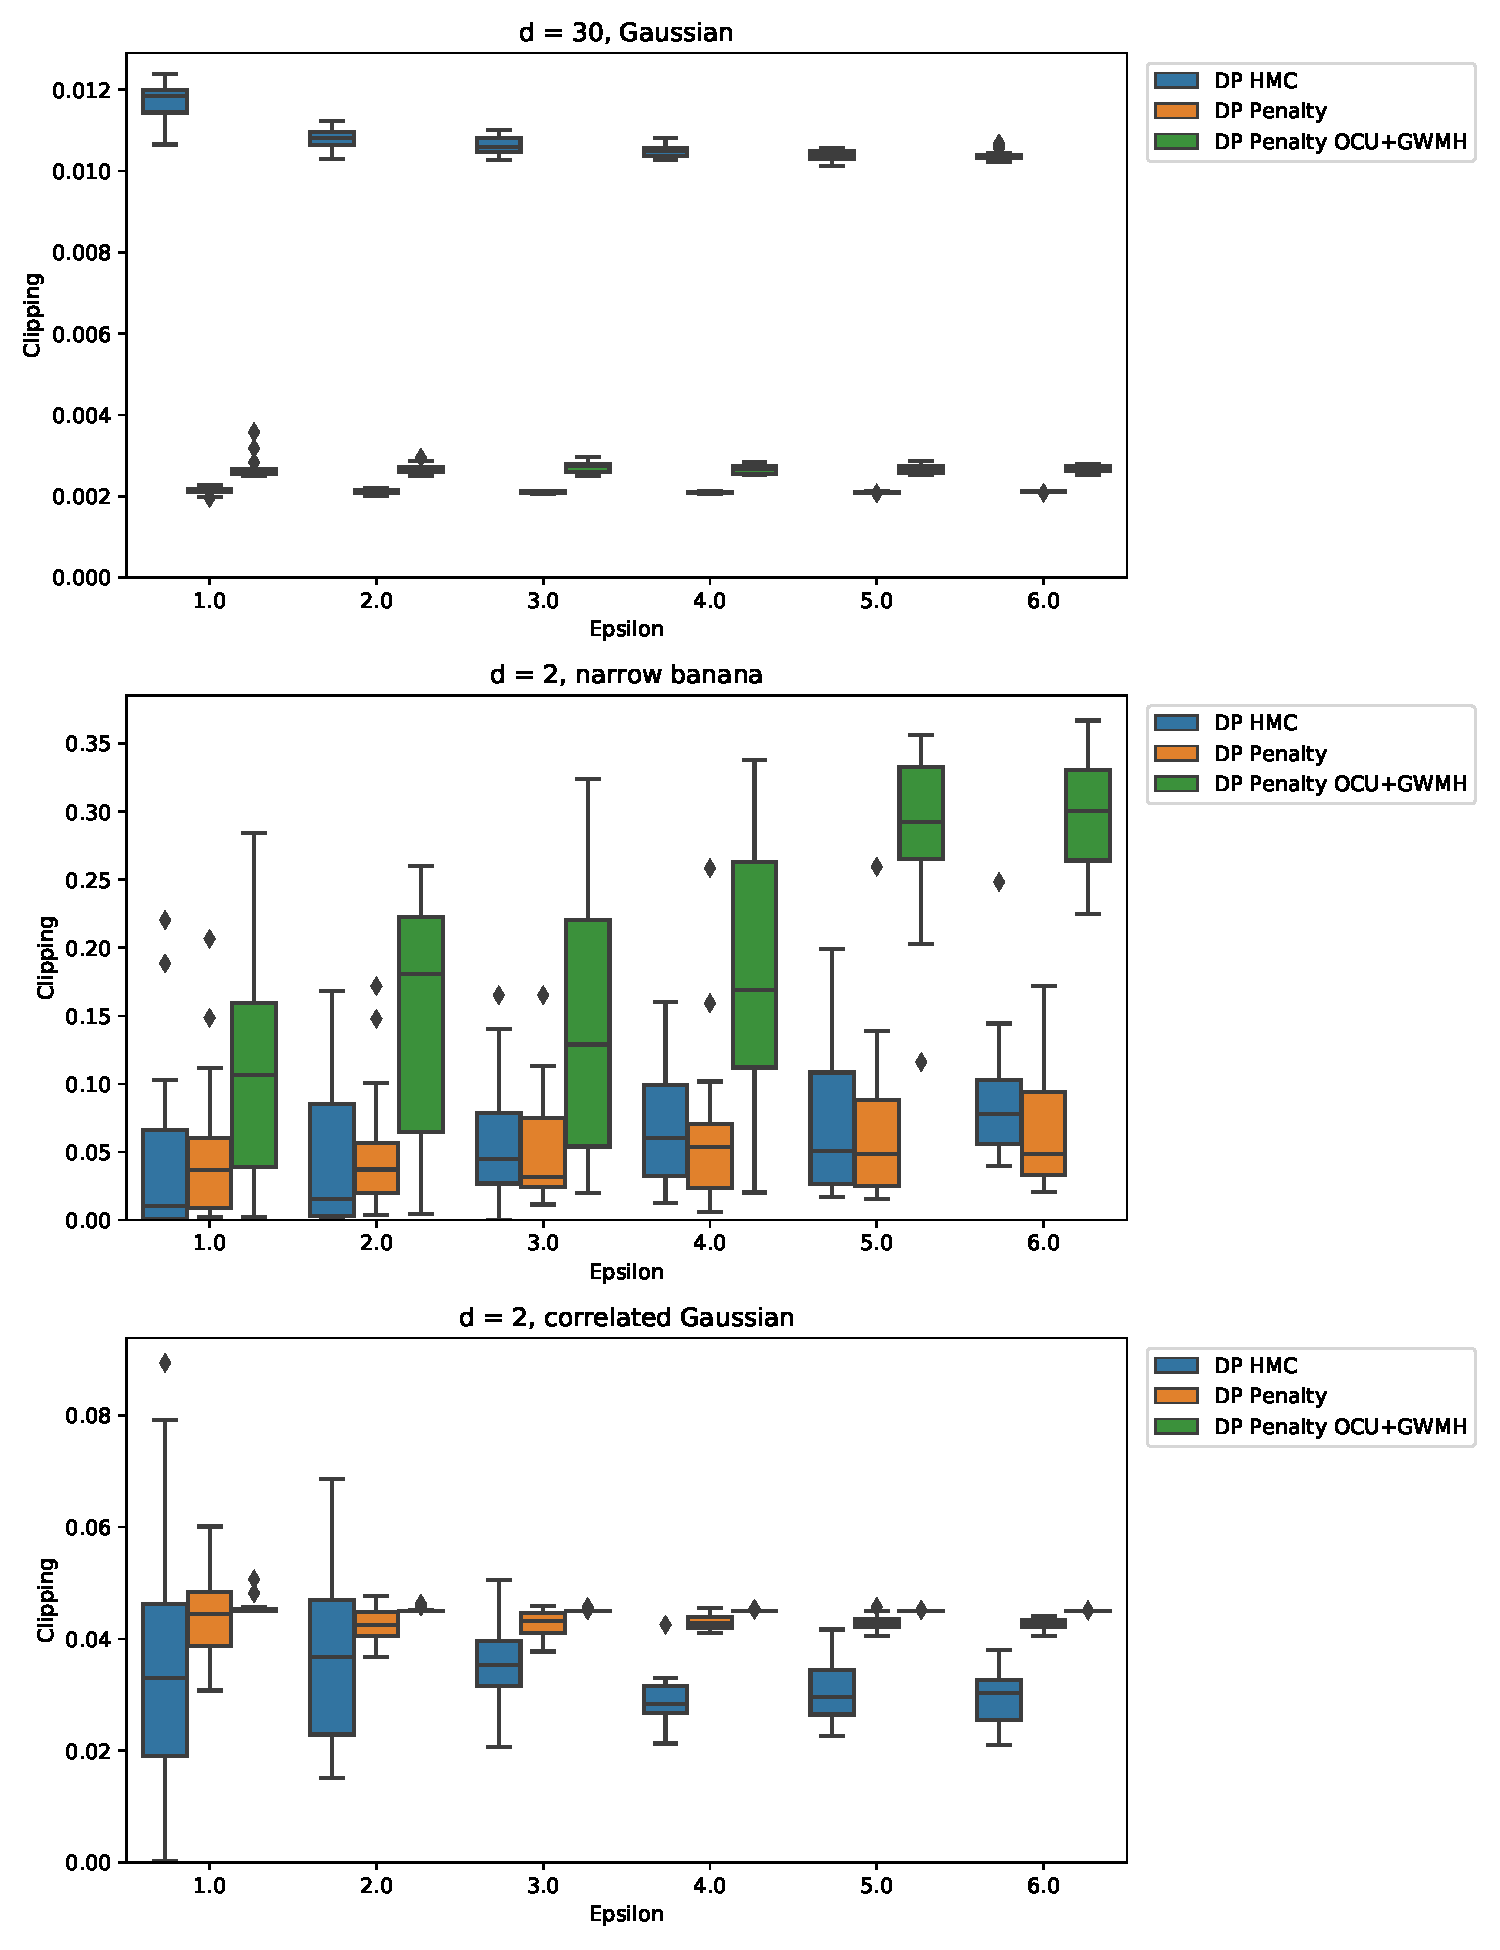
\includegraphics[width=\textwidth]{figures/banana_extra_clipping}
  \caption{
    Clipping for 30-dimensional Gaussian, hard banana and highly correlated
    2-dimensional Gaussian.
  }
  \label{banana_extra_clipping_fig}
\end{figure}

Figure~\ref{circle_fig} shows the results for the circle model. The distance
of the sample mean from the true mean (the origin) were used instead of MMD,
as computing MMD requires a sample from the posterior, which is not trivial
to obtain for the circle model. Both algorithms perform well on average, with
HMC slightly beating DP penalty on \(\epsilon = 0.5\). Clipping is again low
for both algorithms, and HMC has a fairly large variance in clipping between
different runs.

\begin{figure}
  \centering
  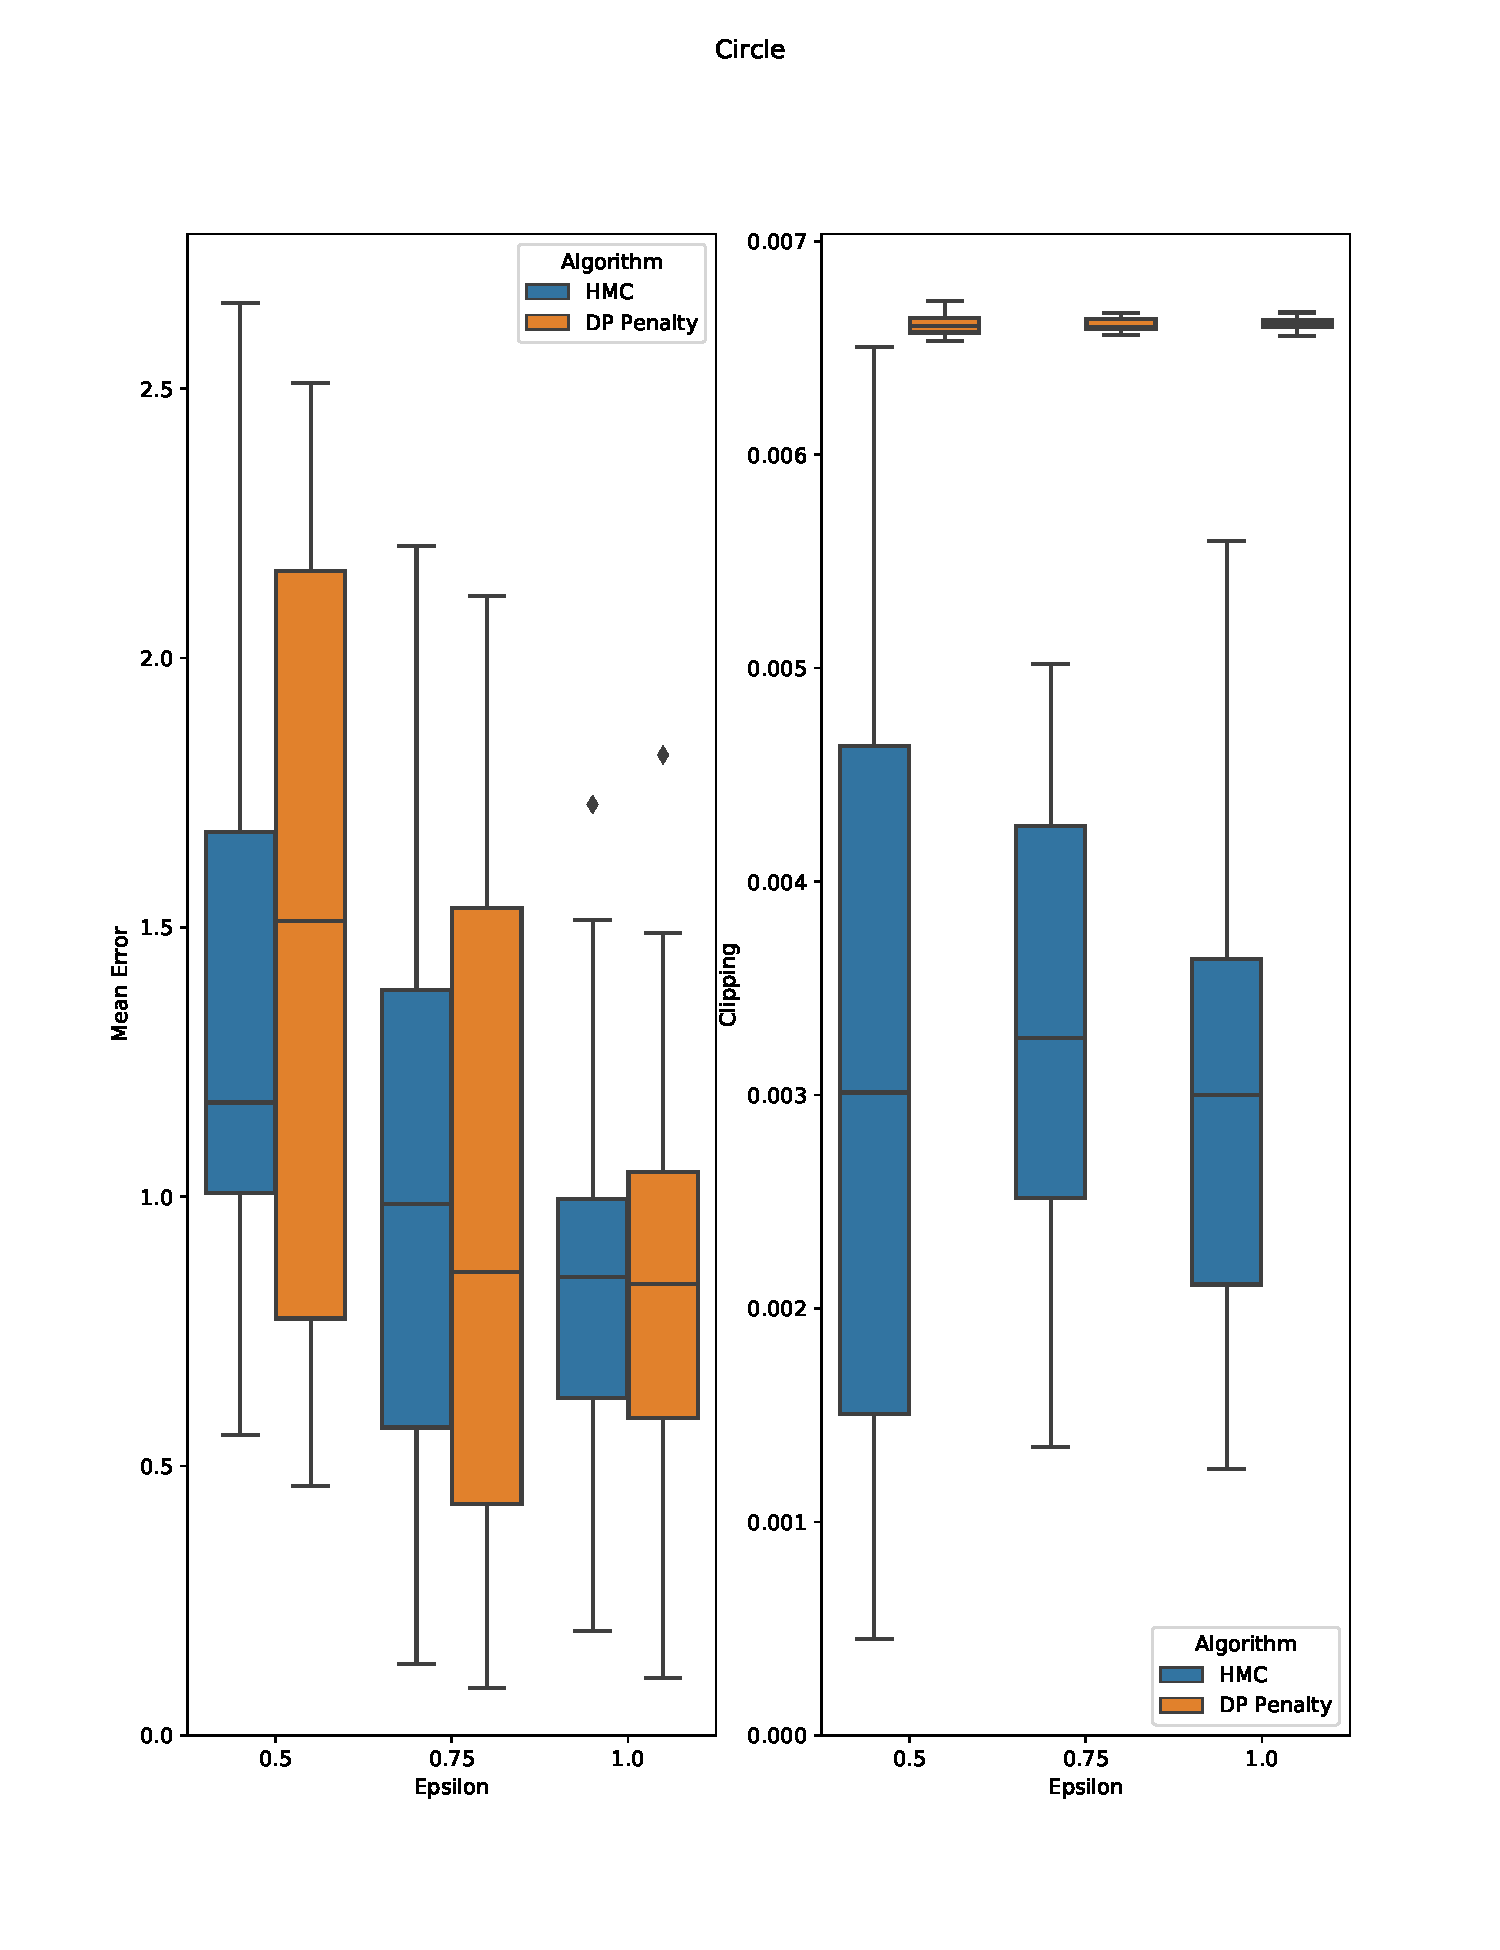
\includegraphics[width=\textwidth]{figures/circle}
  \caption{
    Circle mean error on the left and clipping on the right.
  }
  \label{circle_fig}
\end{figure}

Figure~\ref{grad_clipping_fig} shows the fraction of clipped
gradients for DP HMC. Clipping gradients does not affect the asymptotic
convergence of DP HMC, but it may lower the acceptance rate and thus
the performance of the algorithm. As raising the clip bound to lower
gradient clipping increases the noise added to gradient, thus also lowering
the acceptance rate, it is not clear what an appropriate level of gradient
clipping would be. The observed levels of clipping are fairly constant across
values of \(\epsilon\), but vary in the models, and in the narrow banana model,
there is very large variance in clipping.

\begin{figure}
  \centering
  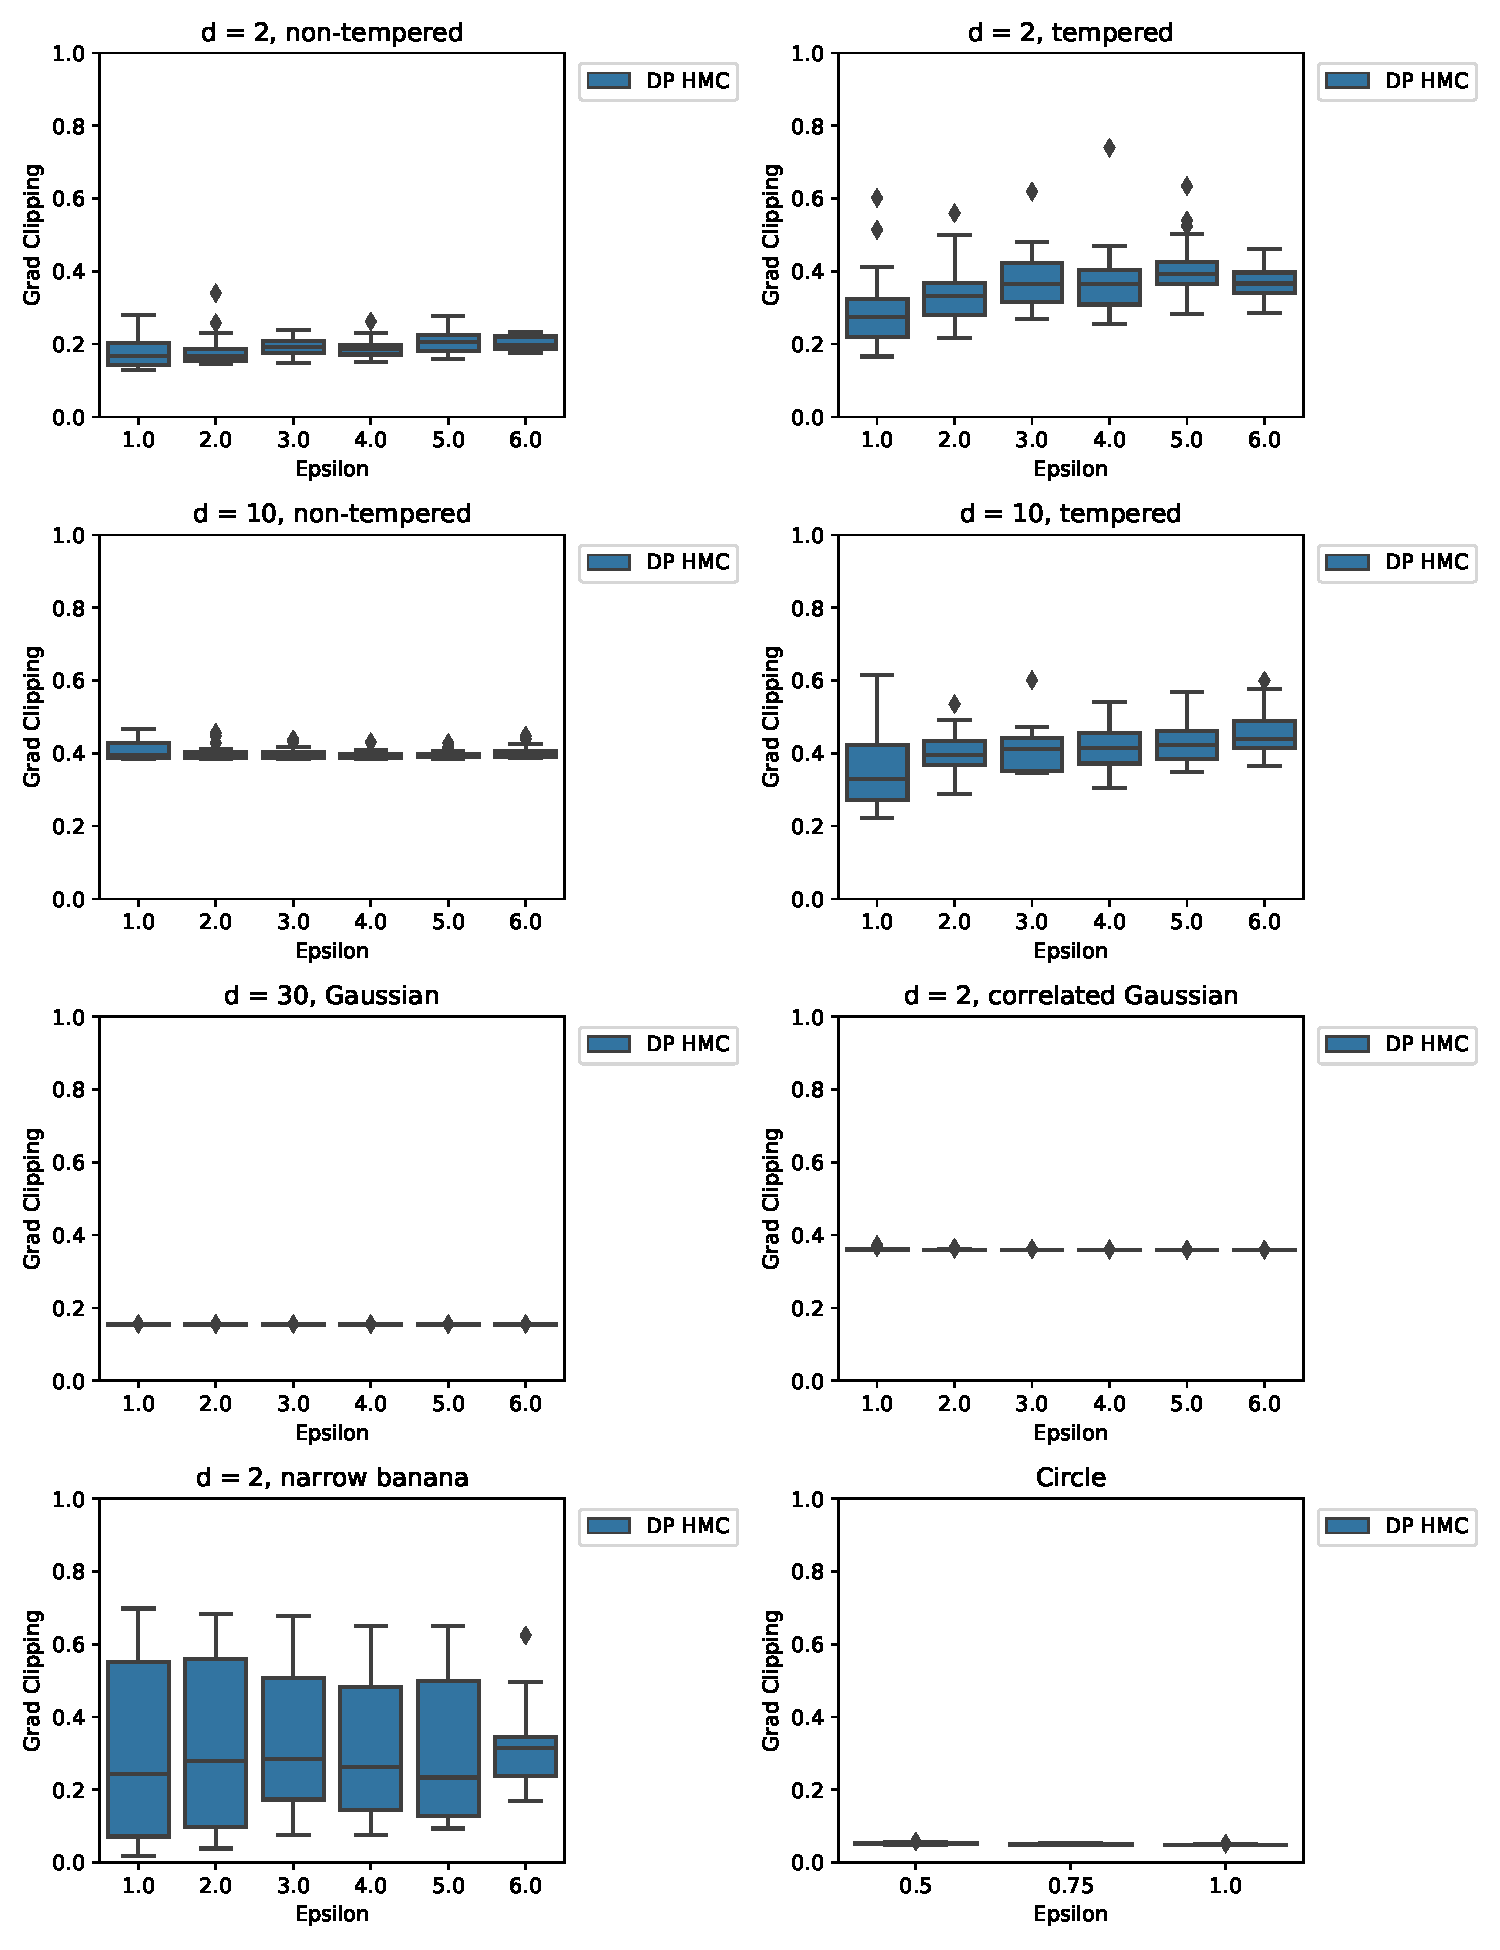
\includegraphics[width=\textwidth]{figures/grad_clipping}
  \caption{
    Gradient clipping for DP HMC.
  }
  \label{grad_clipping_fig}
\end{figure}

\chapter{Conclusions}
% STEP 5:
% Uncomment the following lines and set your .bib file and desired bibliography style
% to make a bibliography with BibTeX.
% Alternatively you can use the thebibliography environment if you want to add all
% references by hand.

\cleardoublepage %fixes the position of bibliography in bookmarks
\phantomsection

\addcontentsline{toc}{chapter}{\bibname} % This lines adds the bibliography to the ToC
\bibliographystyle{alpha} % numbering alphabetic order
\bibliography{../references.bib}

\begin{appendices}
\myappendixtitle

\chapter{Proof of Theorem~\ref{banana_posterior_theorem}}\label{banana_posterior_theorem_proof}

\newcounter{temp_counter}
\setcounter{temp_counter}{\value{theorem}}
\setcounter{theorem}{\value{banana_posterior_theorem_number}}
\addtocounter{theorem}{-1}
\begin{theorem}
    Let
    \begin{align*}
        \theta = (\theta_1,\dotsc, \theta_d) &\sim
        \ban(0, \sigma_0^2I, a, b, m) \\
        X_1 &\sim \caln(\theta_1, \sigma_1^2) \\
        X_2 &\sim \caln(\theta_2 + a(\theta_1 - m)^2 + b, \sigma_2^2)\\
        X_3 &\sim \caln(\theta_3, \sigma_3^2) \\
            &\vdots \\
        X_d &\sim \caln(\theta_d, \sigma_d^2) \\
    \end{align*}
    Given data \(x_1,\dotsc, x_d\in \R^n\) and
    denoting \(\tau_i = \frac{1}{\sigma_i^2}\),
    the posterior of \(\theta\) tempered with \(T\) is the banana distribution
    \(\ban(\mu, \Sigma, a, b, m)\)
    with
    \[
        \bar{x}_i = \frac{1}{n}\sum_{j=1}^n x_{ji} \quad i\in \{1, 2\}
    \]
    \[
        \mu = \left(\frac{Tn\tau_1\bar{x}_1}{Tn\tau_1 + \tau_0},\dotsc,
        \frac{Tn\tau_d\bar{x}_d}{Tn\tau_d + \tau_0}\right),
    \]
    \[
        \Sigma = \diag\left(
            \frac{1}{Tn\tau_1 + \tau_0},\dotsc,
            \frac{1}{Tn\tau_d + \tau_0}
        \right).
    \]
\end{theorem}
\begin{proof}
    Because
    \[
    g^{-1}(y) = (y_1, y_2 + a(y_1 - m)^2 + b, y_3\dotsc, y_d)
    \]
    and the Jacobian determinant of \(g^{-1}\) is \(1\),
    for a positive-definite \(\Sigma\) the banana distribution has
    density proportional to
    \[
    \exp\left(-\frac{1}{2}(g^{-1}(x) - \mu)^T\Sigma^{-1}(g^{-1}(x) - \mu)\right)
    \]
    With \(\Sigma = \diag(\sigma_1^2, \sigma_2^2)\) the density is proportional
    to
    \[
    \exp
    \left(-\frac{1}{2}\left(\left(\frac{x_1 - \mu_1}{\sigma_1}\right)^2
    + \left(\frac{x_2 + a(x_1 - m)^2 + b - \mu_2}{\sigma_2}\right)^2
    + \sum_{i=3}^d\left(\frac{x_i - \mu_i}{\sigma_i}\right)^2\right)\right)
    \]

    Denote \(u = \theta_2 + a(\theta_1 - m)^2 + b\).
    The tempered posterior of \(\theta\) is
    \begin{align*}
        p(\theta\mid X) &\propto p(X\mid \theta)^Tp(\theta)
        \\&= p(X_1\mid \theta_1)^Tp(X_2\mid \theta_1, \theta_2)^T
        \prod_{i=3}^d p(X_i\mid \theta_i)^T p(\theta)
        \\&= p(X_1\mid \theta_1)^Tp(X_2\mid \theta_1, \theta_2)^T
        \prod_{i=3}^d p(X_i\mid \theta_i)^T
        \\&\cdot \exp\left(-\frac{1}{2}\left(\tau_0\theta_1^2
        + \tau_0(\theta_2 + a(\theta_1 - m)^2 + b)^2
        \sum_{i=3}^d \tau_0\theta_i^2\right)\right)
        \\&= p(X_1\mid \theta_1)^Tp(X_2\mid \theta_1, \theta_2)^T
        \exp\left(-\frac{1}{2}\left(\tau_0\theta_1^2
        + \tau_0(\theta_2 + a(\theta_1 - m)^2 + b)^2\right)\right)
        \\&\cdot \prod_{i=3}^d p(X_i\mid \theta_i)^T
        \exp\left(-\frac{1}{2}\sum_{i=3}^d \tau_0\theta_i^2\right)
    \end{align*}

    Considering the upper and lower part of the last expression separately
    \begin{align*}
        &p(X_1\mid \theta_1)^Tp(X_2\mid \theta_1, \theta_2)^T
        \exp\left(-\frac{1}{2}\left(\tau_0\theta_1^2
        + \tau_0(\theta_2 + a(\theta_1 - m)^2 + b)^2\right)\right)
        \\&\propto \left(\prod_{i=1}^n \exp
        \left(-\frac{(x_{i1} - \theta_1)^2\tau_1}{2}\right)\right)^T
        \cdot\left(\prod_{i=1}^n \exp\left(-\frac{(x_{i2} - \theta_2
        - a(\theta_1 - m)^2 - b)^2\tau_2}{2}\right)\right)^T
        \\&\cdot \exp\left(-\frac{1}{2}\left(\tau_0\theta_1^2
        + \tau_0(\theta_2 + a(\theta_1 - m)^2 + b)^2\right)\right)
        \\&=\exp\Bigg(-\frac{1}{2}\Big(T\tau_1\sum_{i=1}^n
        (x_{i1} - \theta_1)^2
        + T\tau_2\sum_{i=1}^n(x_{i2} - u)^2
        + \tau_0\theta_1^2 + \tau_0 u^2\Big)\Bigg)
        \\&=\exp\Bigg(-\frac{1}{2}\Big(T\tau_1\sum_{i=1}^n
        (x_{i1} - \bar{x}_1)^2 + T\tau_1n(\bar{x}_1 - \theta_1)^2
        \\&+ T\tau_2\sum_{i=1}^n (x_{i2}  - \bar{x}_2)^2 + T\tau_2n(\bar{x}_2 - u)^2
        + \tau_0\theta_1^2 + \tau_0 u^2\Big)\Bigg)
        \\&\propto\exp\Bigg(-\frac{1}{2}\Big(T\tau_1n(\bar{x}_1 - \theta_1)^2
        + T\tau_2n(\bar{x}_2 - u)^2
        + \tau_0\theta_1^2 + \tau_0 u^2\Big)\Bigg)
        \\&=\exp\Bigg(-\frac{1}{2}\Big(T\tau_1n\bar{x}_1^2
        - 2T\tau_1n\bar{x}_1\theta_1 + nT\tau_1\theta_1^2 + \tau_0\theta_1^2
        \\&+ T\tau_2n\bar{x}_2^2 - 2T\tau_2n\bar{x}_2u + nT\tau_2u^2
        + \tau_0 u^2\Big)\Bigg)
        \\&\propto\exp\Bigg(-\frac{1}{2}\Big((Tn\tau_1 + \tau_0)\theta_1^2
        - 2T\tau_1n\bar{x}_1\theta_1
        + (Tn\tau_2 + \tau_0)u^2 - 2T\tau_2n\bar{x}_2u \Big)\Bigg)
        \\&=\exp\Bigg(-\frac{1}{2}\Big(
        (Tn\tau_1 + \tau_0)\left(\theta_1^2
        - \frac{2T\tau_1n\bar{x}_1\theta_1}{Tn\tau_1 + \tau_0} \right)
        + (Tn\tau_2 + \tau_0)\left(u^2 - \frac{2T\tau_2n\bar{x}_2u}
        {Tn\tau_2 + \tau_0}\right) \Big)\Bigg)
        \\&\propto\exp\Bigg(-\frac{1}{2}\Big(
        (Tn\tau_1 + \tau_0)\left(\theta_1
        - \frac{T\tau_1n\bar{x}_1}{Tn\tau_1 + \tau_0} \right)^2
        + (Tn\tau_2 + \tau_0)\left(u - \frac{T\tau_2n\bar{x}_2}
        {Tn\tau_2 + \tau_0}\right)^2 \Big)\Bigg)
    \end{align*}
    and
    \begin{align*}
        &\prod_{i=3}^d p(X_i\mid \theta_i)^T
        \cdot \exp\left(-\frac{1}{2}\sum_{i=3}^d \tau_0\theta_i^2\right)
      \\&\propto \exp\left(-\frac{1}{2}T\sum_{j=3}^d\tau_j\sum_{i=1}^n (x_{ij} - \theta_j)^2
      - \frac{1}{2}\sum_{j=3}^d\tau_0\theta_j^2\right)
      \\&= \exp\left(-\frac{1}{2}\sum_{j=3}^d\left(T\tau_j\sum_{i=1}^n (x_{ij} - \theta_j)^2
      + \tau_0\theta_j^2\right)\right)
      \\&= \exp\left(-\frac{1}{2}\sum_{j=3}^d\left(T\tau_j\sum_{i=1}^n (x_{ij} - \bar{x}_j)^2
      + T\tau_j n(\bar{x}_j - \theta_j)^2 + \tau_0\theta_j^2\right)\right)
      \\&\propto \exp\left(-\frac{1}{2}\sum_{j=3}^d\left(T\tau_j n(\bar{x}_j - \theta_j)^2
      + \tau_0\theta_j^2\right)\right)
      \\&\propto \exp\left(-\frac{1}{2}\sum_{j=3}^d\left(
      -2T\tau_j n\bar{x}_j\theta_j + T\tau_jn\theta_j^2
      + \tau_0\theta_j^2\right)\right)
      \\&\propto \exp\left(-\frac{1}{2}\sum_{j=3}^d\left(
      (Tn\tau_j + \tau_0)\theta_j^2
      - 2Tn\tau_j\bar{x}_j\theta_j + \frac{(Tn\tau_j\bar{x}_j)^2}{Tn\tau_j + \tau_0}\right)\right)
      \\&= \exp\left(-\frac{1}{2}\sum_{j=3}^d (Tn\tau_j + \tau_0)\left(\theta_j
      - \frac{Tn\tau_1\bar{x}_i}{Tn\tau_j + \tau_0}\right)^2\right)
    \end{align*}
    Multiplying the resulting expression above gives a density proportional
    to the banana distribution.
    As \(p(\theta\mid X)\) is proportional to the density of a
    banana distribution, the posterior is the banana distribution
    \(\ban(\mu, \Sigma, a, b, m)\)
    with
    \[
        \mu = \left(\frac{Tn\tau_1\bar{x}_1}{Tn\tau_1 + \tau_0},\dotsc,
        \frac{Tn\tau_d\bar{x}_d}{Tn\tau_d + \tau_0}\right),
    \]
    \[
        \Sigma = \diag\left(
            \frac{1}{Tn\tau_1 + \tau_0},\dotsc,
            \frac{1}{Tn\tau_d + \tau_0}
        \right).
        \qedhere
    \]
\end{proof}
\setcounter{theorem}{\value{temp_counter}}

\chapter{Differentiability of the \(\clip\)-function}\label{clip_diff_chapter}

This appendix proves that functions of the form \(\clip\circ f\) are
almost everywhere differentiable for sufficiently well-behaved \(f\),
as required by the proof of volume preservation
of DP HMC leapfrog iterations (Section~\ref{dp_hmc_section}).
Lemma~\ref{clip_is_almost_everywhere_differentiable} gives very general
sufficient conditions, and Lemma~\ref{model_clip_ok_lemma} proves that the
models considered in this thesis meet the conditions.

\begin{lemma}\label{level_set_lemma}
  Let \(d \geq 2\) and \(g\colon U \to \R\), where \(U\) is an open subset of
  \(\R^{d}\), be continuously differentiable. Let \(S = \{x\in U\mid f(x) = b\}\),
  \(b\in \R\).
  If for all \(x\in S\), \(\nabla f(x) \neq 0\), \(S\) is a \((d - 1)\)-dimensional
  hypersurface.
\end{lemma}
\begin{proof}
	See~\cite[Section 9.2]{Tu11}.
\end{proof}

\begin{lemma}\label{clip_is_almost_everywhere_differentiable}
  Let \(f\colon \R^{d}\to \R^{d}\) be continuously differentiable.
  If the set of saddle points \(U\) of \(||f||\) is a null set,
  the set \(A\subset \R^{d}\)
  where \(\clip_{b} \circ f\) is not differentiable is a null set.
\end{lemma}
\begin{proof}
  \[
    \clip_{b}(x) = \frac{x}{||x||}\min\{||x||, b\}
  \]
  which means that \(\clip_{b}\) is differentiable for all \(x\in \R^{d}\) with
  \(||x|| \neq b\). Consider \(\clip_{b}\circ f\) in a neighbourhood \(B\) of
  point \(x_{0}\in \R^{d}\). If \(||f(x)|| \leq b\) for all \(x\in B\),
  \(\clip_{b}(f(x)) = f(x)\) in \(B\), which is differentiable. If \(||f(x)|| \geq b\)
  for all \(x\in B\), \(\clip_{b}(f(x)) = \frac{f(x)b}{||f(x)||}\) in \(B\),
  which is also differentiable because \(f(x) \neq 0\) when
  \(||f(x)|| \geq b > 0\). In both cases \(\clip_{b}\circ f\) is differentiable
  at \(x_{0}\). This means that for all \(x_{0}\in A\), \(||f(x_{0})|| = b\), but
  every neighborhood
  of \(x_{0}\) has points \(x'\) and \(x''\) such that \(||f(x')|| < b\) and
  \(||f(x'')|| > b\). With the differentiability of \(f\), this means that
  if \(\nabla ||f(x_{0})|| = 0\), \(x_{0}\) is a saddle point of \(||f||\).

  Let \(S = \{x\in \R^{d}\mid ||f(x)|| = b \text{ and } \nabla ||f(x)|| \neq 0\}\).
  % With the assumptions on \(f\),
  % there is a neighborhood \(E\subset U\)
  % for every \(x_{0}\in S\) where \(f(x) \neq 0\) for all \(x\in E\) and
  % \(||f||\) is differentiable.
  % \(\nabla ||f(x)|| = \frac{2f(x)}{||f(x)||}J_{f}(x) \neq 0\) for \(x\in S\).
  By Lemma~\ref{level_set_lemma},
  \(S\) is a \((d-1)\)-dimensional hypersurface, which has zero measure
  in \(d\)-dimensional space. Because \(A\cap U^{C} \subset S\), \(A\cap U^{C}\)
  is also a null set. Since \(A = (A\cap U^{C}) \cup (A\cap U)\),
  \(A\) is a null set.

  % Let \(E(x_{1}) = \{(x_{2}, \dotsc, \x_{d})\in \R^{d-1}\mid (x_{1}\dotsc, x_{d})\in A\}\).
  % \(E(x_{1})\) has measure zero for almost all \(x_{1}\).

  % Let \(x_{1}\in \R\) where \(E(x_{1})\) has non-zero measure.
\end{proof}

For DP HMC, set \(f(\theta) = \nabla U(\theta)\). The conditions of
Lemma~\ref{clip_is_almost_everywhere_differentiable} for \(U\) are met if
\(U\) is twice continuously differentiable and
\begin{lemma}\label{model_clip_ok_lemma}
  The log-likelihoods of the Gaussian, banana and circle models meet the
  conditions of Lemma~\ref{clip_is_almost_everywhere_differentiable}.
\end{lemma}
\begin{proof}
For DP HMC, set \(f(\theta) = \nabla U(\theta)\). The conditions of
Lemma~\ref{clip_is_almost_everywhere_differentiable} for \(U\) are met if
\(U\) is twice continuously differentiable and
\[
  \nabla ||\nabla U(x)||
  = \frac{2\nabla U(x)}{||\nabla U(x)||}J_{\nabla U}(x)
  = \frac{2\nabla U(x)}{||\nabla U(x)||}H_{U}(x) \neq 0
\]
almost everywhere,
where \(H_{U}\) is the Hessian matrix of \(U\). Because \(\nabla U = 0\) and
\(||\nabla U|| = 0\) at only one point, having \(\det H_{U}(x) \neq 0\)
almost everywhere is sufficient.

For the Gaussian log-likelihood
\[
  U(\theta) = \frac{1}{2}(x - \theta)^{T}\Sigma^{-1}(x - \theta),
\]
so
\[
  \nabla U(\theta) = \Sigma^{-1}(x - \theta)
\]
and \(H_{U}(\theta) = \Sigma^{-1}\).

For the banana log-likelihood, using the notation from
Appendix~\ref{banana_posterior_theorem_proof},
\[
  U(\theta) = \frac{1}{2}(g^{-1}(x) - \theta)^{T}\Sigma^{-1}(g^{-1}(x) - \theta),
\]
so
\[
  \nabla U(\theta) = \Sigma^{-1}(g^{-1}(x) - \theta)
\]
and \(H_{U}(\theta) = \Sigma^{-1}\).

The circle log-likelihood is
\[
  U(x, y) = -a(x^{2} + y^{2} - r^{2})^{2},
\]
\[
  \nabla U(x, y) = -4a(x^{3} + xy^{2} - xr^{2}, x^{2}y + y^{3} - yr^{2}),
\]
so
\[
  H_{U}(x, y) = -4a
  \begin{bmatrix}
    3x^{2} + y^{2} - r^{2} & 2xy \\
    2xy & 3y^{2} + x^{2} - r^{2} \\
  \end{bmatrix}
\]
and
\begin{align*}
  \det H_{U}(x, y) &= -4a((3x^{2} + y^{2} - r^{2})(3y^{2} + x^{2} - r^{2})
  - 4x^{2}y^{2})
  \\&= -4a(9x^{2}y^{2} + 3x^{4} - 3x^{2}r^{2} + 3y^{4} + y^{2}x^{2} -y^{2}r^{2}
  - 3y^{2}r^{2} - x^{2}r^{2} + r^{4} - 4x^{2}y^{2})
  \\&= -4a(6x^{2}y^{2} + 3x^{4} - 4x^{2}r^{2} + 3y^{4} - 4y^{2}r^{2} + r^{4})
  \\&= -4a(6x^{2}y^{2} + 3(x^{4} + y^{4}) - 4r^{2}(x^{2} + y^{2}) + r^{4}).
\end{align*}
\[
  \nabla \det H_{U}(x, y) = -4a(12xy^{2} + 12x^{3} - 8r^{2}x,
  12yx^{2} + 12y^{3} - 8r^{2}y),
\]
which is zero in the origin and on the circle
\[
  x^{2} + y^{2} = \frac{2}{3}r^{2}.
\]
Elsewhere, Lemma~\ref{level_set_lemma} can be applied to \(\det H_{U}\), which
means that the set where \(\det H_{U}(x, y) = 0\) is a 1-dimensional curve.
\end{proof}
\end{appendices}

\end{document}
